% Options for packages loaded elsewhere
\PassOptionsToPackage{unicode=true}{hyperref}
\PassOptionsToPackage{hyphens}{url}
%
\documentclass[
]{article}
\usepackage{lmodern}
\usepackage{amssymb,amsmath}
\usepackage{ifxetex,ifluatex}
\ifnum 0\ifxetex 1\fi\ifluatex 1\fi=0 % if pdftex
  \usepackage[T1]{fontenc}
  \usepackage[utf8]{inputenc}
  \usepackage{textcomp} % provides euro and other symbols
\else % if luatex or xelatex
  \usepackage{unicode-math}
  \defaultfontfeatures{Scale=MatchLowercase}
  \defaultfontfeatures[\rmfamily]{Ligatures=TeX,Scale=1}
\fi
% Use upquote if available, for straight quotes in verbatim environments
\IfFileExists{upquote.sty}{\usepackage{upquote}}{}
\IfFileExists{microtype.sty}{% use microtype if available
  \usepackage[]{microtype}
  \UseMicrotypeSet[protrusion]{basicmath} % disable protrusion for tt fonts
}{}
\makeatletter
\@ifundefined{KOMAClassName}{% if non-KOMA class
  \IfFileExists{parskip.sty}{%
    \usepackage{parskip}
  }{% else
    \setlength{\parindent}{0pt}
    \setlength{\parskip}{6pt plus 2pt minus 1pt}}
}{% if KOMA class
  \KOMAoptions{parskip=half}}
\makeatother
\usepackage{xcolor}
\IfFileExists{xurl.sty}{\usepackage{xurl}}{} % add URL line breaks if available
\IfFileExists{bookmark.sty}{\usepackage{bookmark}}{\usepackage{hyperref}}
\hypersetup{
  pdftitle={Fluent genomics with plyranges and tximeta},
  pdfauthor={Stuart Lee, Michael Lawrence, Michael Love},
  hidelinks,
}
\urlstyle{same} % disable monospaced font for URLs
\usepackage[margin=1in]{geometry}
\usepackage{color}
\usepackage{fancyvrb}
\newcommand{\VerbBar}{|}
\newcommand{\VERB}{\Verb[commandchars=\\\{\}]}
\DefineVerbatimEnvironment{Highlighting}{Verbatim}{commandchars=\\\{\}}
% Add ',fontsize=\small' for more characters per line
\newenvironment{Shaded}{}{}
\newcommand{\AlertTok}[1]{\textcolor[rgb]{1.00,0.00,0.00}{\textbf{#1}}}
\newcommand{\AnnotationTok}[1]{\textcolor[rgb]{0.38,0.63,0.69}{\textbf{\textit{#1}}}}
\newcommand{\AttributeTok}[1]{\textcolor[rgb]{0.49,0.56,0.16}{#1}}
\newcommand{\BaseNTok}[1]{\textcolor[rgb]{0.25,0.63,0.44}{#1}}
\newcommand{\BuiltInTok}[1]{#1}
\newcommand{\CharTok}[1]{\textcolor[rgb]{0.25,0.44,0.63}{#1}}
\newcommand{\CommentTok}[1]{\textcolor[rgb]{0.38,0.63,0.69}{\textit{#1}}}
\newcommand{\CommentVarTok}[1]{\textcolor[rgb]{0.38,0.63,0.69}{\textbf{\textit{#1}}}}
\newcommand{\ConstantTok}[1]{\textcolor[rgb]{0.53,0.00,0.00}{#1}}
\newcommand{\ControlFlowTok}[1]{\textcolor[rgb]{0.00,0.44,0.13}{\textbf{#1}}}
\newcommand{\DataTypeTok}[1]{\textcolor[rgb]{0.56,0.13,0.00}{#1}}
\newcommand{\DecValTok}[1]{\textcolor[rgb]{0.25,0.63,0.44}{#1}}
\newcommand{\DocumentationTok}[1]{\textcolor[rgb]{0.73,0.13,0.13}{\textit{#1}}}
\newcommand{\ErrorTok}[1]{\textcolor[rgb]{1.00,0.00,0.00}{\textbf{#1}}}
\newcommand{\ExtensionTok}[1]{#1}
\newcommand{\FloatTok}[1]{\textcolor[rgb]{0.25,0.63,0.44}{#1}}
\newcommand{\FunctionTok}[1]{\textcolor[rgb]{0.02,0.16,0.49}{#1}}
\newcommand{\ImportTok}[1]{#1}
\newcommand{\InformationTok}[1]{\textcolor[rgb]{0.38,0.63,0.69}{\textbf{\textit{#1}}}}
\newcommand{\KeywordTok}[1]{\textcolor[rgb]{0.00,0.44,0.13}{\textbf{#1}}}
\newcommand{\NormalTok}[1]{#1}
\newcommand{\OperatorTok}[1]{\textcolor[rgb]{0.40,0.40,0.40}{#1}}
\newcommand{\OtherTok}[1]{\textcolor[rgb]{0.00,0.44,0.13}{#1}}
\newcommand{\PreprocessorTok}[1]{\textcolor[rgb]{0.74,0.48,0.00}{#1}}
\newcommand{\RegionMarkerTok}[1]{#1}
\newcommand{\SpecialCharTok}[1]{\textcolor[rgb]{0.25,0.44,0.63}{#1}}
\newcommand{\SpecialStringTok}[1]{\textcolor[rgb]{0.73,0.40,0.53}{#1}}
\newcommand{\StringTok}[1]{\textcolor[rgb]{0.25,0.44,0.63}{#1}}
\newcommand{\VariableTok}[1]{\textcolor[rgb]{0.10,0.09,0.49}{#1}}
\newcommand{\VerbatimStringTok}[1]{\textcolor[rgb]{0.25,0.44,0.63}{#1}}
\newcommand{\WarningTok}[1]{\textcolor[rgb]{0.38,0.63,0.69}{\textbf{\textit{#1}}}}
\usepackage{longtable,booktabs}
% Allow footnotes in longtable head/foot
\IfFileExists{footnotehyper.sty}{\usepackage{footnotehyper}}{\usepackage{footnote}}
\makesavenoteenv{longtable}
\usepackage{graphicx,grffile}
\makeatletter
\def\maxwidth{\ifdim\Gin@nat@width>\linewidth\linewidth\else\Gin@nat@width\fi}
\def\maxheight{\ifdim\Gin@nat@height>\textheight\textheight\else\Gin@nat@height\fi}
\makeatother
% Scale images if necessary, so that they will not overflow the page
% margins by default, and it is still possible to overwrite the defaults
% using explicit options in \includegraphics[width, height, ...]{}
\setkeys{Gin}{width=\maxwidth,height=\maxheight,keepaspectratio}
\setlength{\emergencystretch}{3em} % prevent overfull lines
\providecommand{\tightlist}{%
  \setlength{\itemsep}{0pt}\setlength{\parskip}{0pt}}
\setcounter{secnumdepth}{5}
% Redefines (sub)paragraphs to behave more like sections
\ifx\paragraph\undefined\else
  \let\oldparagraph\paragraph
  \renewcommand{\paragraph}[1]{\oldparagraph{#1}\mbox{}}
\fi
\ifx\subparagraph\undefined\else
  \let\oldsubparagraph\subparagraph
  \renewcommand{\subparagraph}[1]{\oldsubparagraph{#1}\mbox{}}
\fi

% Set default figure placement to htbp
\makeatletter
\def\fps@figure{htbp}
\makeatother


\title{Fluent genomics with plyranges and tximeta}
\author{Stuart Lee, Michael Lawrence, Michael Love}
\date{}

\begin{document}
\maketitle
\begin{abstract}
We construct a simple workflow for fluent genomics data analysis using the R/Bioconductor ecosystem. This involves three core steps: \textbf{import} the data into an appropriate abstraction, \textbf{model} the data with respect to the biological questions of interest, and \textbf{integrate} the results with respect to their underlying genomic coordinates. Here we show how to implement these steps to integrate published RNA-seq and ATAC-seq experiments on macrophage cell lines. Using \emph{tximeta}, we \textbf{import} RNA-seq transcript quantifications into an analysis-ready data structure, called the \emph{SummarizedExperiment}, that contains the ranges of the reference transcripts and metadata on their provenance. Using \emph{SummarizedExperiment}s to represent the ATAC-seq and RNA-seq data, we \textbf{model} differentially accessible (DA) chromatin peaks and differentially expressed (DE) genes with existing Bioconductor packages. Using \emph{plyranges} we then \textbf{integrate} the results to see if there is an enrichment of DA peaks near DE genes by finding overlaps and aggregating over log-fold change thresholds. The combination of these packages and their integration with the Bioconductor ecosystem provide a coherent framework for analysts to iteratively and reproducibly explore their biological data.
\end{abstract}



























\hypertarget{introduction}{%
\section{Introduction}\label{introduction}}

In this workflow, we examine a subset of the RNA-seq and ATAC-seq data from
K Alasoo et al. (\protect\hyperlink{ref-alasoo}{2018}), a study that involved treatment of macrophage cell lines from a number
of human donors with interferon gamma (IFNg), \emph{Salmonella} infection, or both
treatments combined. K Alasoo et al. (\protect\hyperlink{ref-alasoo}{2018}) examined gene expression and chromatin
accessibility in a subset of 86 successfully differentiated induced pluripotent
stem cells (iPSC) lines, and compared baseline and response with respect to
chromatin accessibility and gene expression at specific quantitative trait loci
(QTL). The authors found that many of the stimulus-specific expression QTL were
already detectable as chromatin QTL in naive cells, and further hypothesize
about the nature and role of transcription factors implicated in the response
to stimulus.

We will perform a much simpler analysis than the one found in K Alasoo et al. (\protect\hyperlink{ref-alasoo}{2018}), using
their publicly available RNA-seq and ATAC-seq data (ignoring the genotypes). We
will examine the effect of IFNg stimulation on gene expression and chromatin
accessibility, and look to see if there is an enrichment of differentially
accessible (DA) ATAC-seq peaks in the vicinity of differentially expressed (DE)
genes. This is plausible, as the transcriptomic response to IFNg stimulation
may be mediated through binding of regulatory proteins to accessible regions,
and this binding may increase the accessibility of those regions such that it
can be detected by ATAC-seq.

\begin{figure}

{\centering 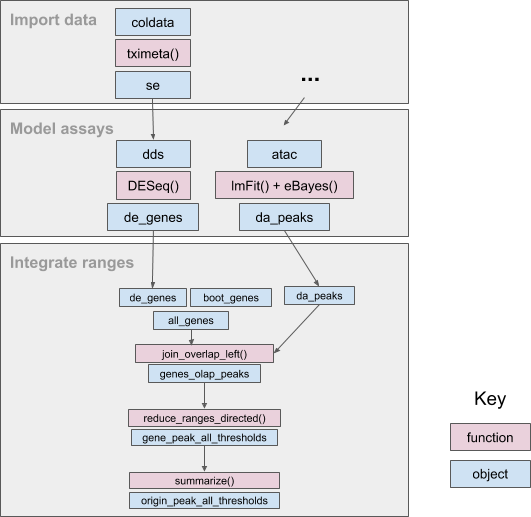
\includegraphics[width=\textwidth]{workflow} 

}

\caption{An overview of the fluent genomics workflow. First, we \emph{import}
data as a \emph{SummarizedExperiment} object, which enables interoperability with
downstream analysis packages. Then we \emph{model} our assay data, using the
existing Bioconductor packages \emph{DESeq2} and \emph{limma}. We take the results of our
models for each assay with respect to their genomic coordinates, and
\emph{integrate} them. First, we compute the overlap between the results of each
assay, then aggregate over the combined genomic regions, and finally summarize
to compare enrichment for differentially expressed genes to non differentially
expressed genes. The final output can be used for downstream visualization or
further transformation.}\label{fig:workflow}
\end{figure}

Throughout the workflow (Figure \ref{fig:workflow}), we will use existing
Bioconductor infrastructure to understand these datasets. In particular, we
will emphasize the use of the Bioconductor packages \emph{plyranges} and \emph{tximeta}.
The \emph{plyranges} package fluently transforms data tied to genomic ranges using
operations like shifting, window construction, overlap detection, etc. It is
described by Lee, Cook, and Lawrence (\protect\hyperlink{ref-Lee2019}{2019}) and leverages underlying core Bioconductor infrastructure
(Lawrence et al. \protect\hyperlink{ref-granges}{2013}; Huber et al. \protect\hyperlink{ref-bioc}{2015}) and the \emph{tidyverse} design principles Wickham et al. (\protect\hyperlink{ref-tidyverse}{2019}).

The \emph{tximeta} package described by Love et al. (\protect\hyperlink{ref-Love2019-tximeta}{2019}) is used to read RNA-seq
quantification data into R/Bioconductor, such that the transcript ranges and
their provenance are automatically attached to the object containing expression
values and differential expression results.

\hypertarget{experimental-data}{%
\subsection{Experimental Data}\label{experimental-data}}

The data used in this workflow is available from two packages: the \emph{macrophage}
Bioconductor ExperimentData package and from the workflow package
\emph{fluentGenomics}.

The \emph{macrophage} package contains RNA-seq quantification from 24 RNA-seq
samples, a subset of the RNA-seq samples generated and analyzed by K Alasoo et al. (\protect\hyperlink{ref-alasoo}{2018}). The
paired-end reads were quantified using \emph{Salmon} (R. Patro et al. \protect\hyperlink{ref-salmon}{2017}), using the Gencode 29
human reference transcripts (Frankish, GENCODE-consoritum, and Flicek \protect\hyperlink{ref-gencode}{2018}). For more details on quantification, and
the exact code used, consult the vignette of the
\href{http://bioconductor.org/packages/macrophage}{macrophage} package. The package
also contains the \texttt{Snakemake} file that was used to distribute the \emph{Salmon}
quantification jobs on a cluster (Köster and Rahmann \protect\hyperlink{ref-snakemake}{2012}).

The \emph{fluentGenomics} package contains functionality to download and generate a
cached \emph{SummarizedExperiment} object from the normalized ATAC-seq data provided
by Kaur Alasoo and Gaffney (\protect\hyperlink{ref-alasooZenodo}{2017}). This object contains all 145 ATAC-seq samples across all
experimental conditions as analyzed by K Alasoo et al. (\protect\hyperlink{ref-alasoo}{2018}). The data can be also be
downloaded directly from the
\href{https://zenodo.org/record/1188300\#.XIAhXlNKjOQ}{Zenodo} deposition.

The following code loads the path to the cached data file, or if it is not
present, will create the cache and generate a \emph{SummarizedExperiment} using the
the \emph{BiocFileCache} package (Shepherd and Morgan \protect\hyperlink{ref-bcfilecache}{2019}).

\begin{Shaded}
\begin{Highlighting}[]
\KeywordTok{library}\NormalTok{(fluentGenomics)}
\NormalTok{path_to_se <-}\StringTok{ }\KeywordTok{cache_atac_se}\NormalTok{()}
\end{Highlighting}
\end{Shaded}

We can then read the cached file and assign it to an object called \texttt{atac}.

\begin{Shaded}
\begin{Highlighting}[]
\NormalTok{atac <-}\StringTok{ }\KeywordTok{readRDS}\NormalTok{(path_to_se)}
\end{Highlighting}
\end{Shaded}

A precise description of how we obtained this \emph{SummarizedExperiment} object can
be found in section \ref{atac}.

\hypertarget{se}{%
\section{\texorpdfstring{Import Data as a \emph{SummarizedExperiment}}{Import Data as a SummarizedExperiment}}\label{se}}

\hypertarget{using-tximeta-to-import-rna-seq-quantification-data}{%
\subsection{\texorpdfstring{Using \emph{tximeta} to import RNA-seq quantification data}{Using tximeta to import RNA-seq quantification data}}\label{using-tximeta-to-import-rna-seq-quantification-data}}

First, we specify a directory \texttt{dir}, where the quantification files are stored.
You could simply specify this directory with:

\begin{Shaded}
\begin{Highlighting}[]
\NormalTok{dir <-}\StringTok{ "/path/to/quant/files"}
\end{Highlighting}
\end{Shaded}

where the path is relative to your current R session. However, in this case we
have distributed the files in the \emph{macrophage} package. The relevant directory
and associated files can be located using \texttt{system.file}.

\begin{Shaded}
\begin{Highlighting}[]
\NormalTok{dir <-}\StringTok{ }\KeywordTok{system.file}\NormalTok{(}\StringTok{"extdata"}\NormalTok{, }\DataTypeTok{package=}\StringTok{"macrophage"}\NormalTok{)}
\end{Highlighting}
\end{Shaded}

Information about the experiment is contained in the \texttt{coldata.csv} file. We
leverage the \emph{dplyr} and \emph{readr} packages (as part of the \emph{tidyverse}) to read
this file into R (Wickham et al. \protect\hyperlink{ref-tidyverse}{2019}). We will see later that \emph{plyranges} extends these
packages to accommodate genomic ranges.

\begin{Shaded}
\begin{Highlighting}[]
\KeywordTok{library}\NormalTok{(dplyr)}
\end{Highlighting}
\end{Shaded}

\begin{verbatim}
## 
## Attaching package: 'dplyr'
\end{verbatim}

\begin{verbatim}
## The following objects are masked from 'package:stats':
## 
##     filter, lag
\end{verbatim}

\begin{verbatim}
## The following objects are masked from 'package:base':
## 
##     intersect, setdiff, setequal, union
\end{verbatim}

\begin{Shaded}
\begin{Highlighting}[]
\KeywordTok{library}\NormalTok{(readr)}
\NormalTok{colfile <-}\StringTok{ }\KeywordTok{file.path}\NormalTok{(dir, }\StringTok{"coldata.csv"}\NormalTok{)}
\NormalTok{coldata <-}\StringTok{ }\KeywordTok{read_csv}\NormalTok{(colfile) }\OperatorTok
\StringTok{  }\NormalTok{dplyr}\OperatorTok{::}\KeywordTok{select}\NormalTok{(}
\NormalTok{    names,}
    \DataTypeTok{id =}\NormalTok{ sample_id,}
    \DataTypeTok{line =}\NormalTok{ line_id,}
    \DataTypeTok{condition =}\NormalTok{ condition_name}
\NormalTok{  ) }\OperatorTok
\StringTok{  }\NormalTok{dplyr}\OperatorTok{::}\KeywordTok{mutate}\NormalTok{(}
    \DataTypeTok{files =} \KeywordTok{file.path}\NormalTok{(dir, }\StringTok{"quants"}\NormalTok{, names, }\StringTok{"quant.sf.gz"}\NormalTok{),}
    \DataTypeTok{line =} \KeywordTok{factor}\NormalTok{(line),}
    \DataTypeTok{condition =} \KeywordTok{relevel}\NormalTok{(}\KeywordTok{factor}\NormalTok{(condition), }\StringTok{"naive"}\NormalTok{)}
\NormalTok{  )}
\end{Highlighting}
\end{Shaded}

\begin{verbatim}
## Parsed with column specification:
## cols(
##   names = col_character(),
##   sample_id = col_character(),
##   line_id = col_character(),
##   replicate = col_double(),
##   condition_name = col_character(),
##   macrophage_harvest = col_character(),
##   salmonella_date = col_character(),
##   ng_ul_mean = col_double(),
##   rna_extraction = col_character(),
##   rna_submit = col_character(),
##   library_pool = col_character(),
##   chemistry = col_character(),
##   rna_auto = col_double()
## )
\end{verbatim}

\begin{Shaded}
\begin{Highlighting}[]
\NormalTok{coldata}
\end{Highlighting}
\end{Shaded}

\begin{verbatim}
## # A tibble: 24 x 5
##    names      id     line  condition  files                                     
##    <chr>      <chr>  <fct> <fct>      <chr>                                     
##  1 SAMEA1038~ diku_A diku~ naive      /Library/Frameworks/R.framework/Versions/~
##  2 SAMEA1038~ diku_B diku~ IFNg       /Library/Frameworks/R.framework/Versions/~
##  3 SAMEA1038~ diku_C diku~ SL1344     /Library/Frameworks/R.framework/Versions/~
##  4 SAMEA1038~ diku_D diku~ IFNg_SL13~ /Library/Frameworks/R.framework/Versions/~
##  5 SAMEA1038~ eiwy_A eiwy~ naive      /Library/Frameworks/R.framework/Versions/~
##  6 SAMEA1038~ eiwy_B eiwy~ IFNg       /Library/Frameworks/R.framework/Versions/~
##  7 SAMEA1038~ eiwy_C eiwy~ SL1344     /Library/Frameworks/R.framework/Versions/~
##  8 SAMEA1038~ eiwy_D eiwy~ IFNg_SL13~ /Library/Frameworks/R.framework/Versions/~
##  9 SAMEA1038~ fikt_A fikt~ naive      /Library/Frameworks/R.framework/Versions/~
## 10 SAMEA1038~ fikt_B fikt~ IFNg       /Library/Frameworks/R.framework/Versions/~
## # ... with 14 more rows
\end{verbatim}

After we have read the \texttt{coldata.csv} file, we select relevant columns from this
table, create a new column called \texttt{files}, and transform the existing \texttt{line}
and \texttt{condition} columns into factors. In the case of \texttt{condition}, we specify
the ``naive'' cell line as the reference level. The \texttt{files} column points to the
quantifications for each observation -- these files have been gzipped, but
would typically not have the `gz' ending if used from \emph{Salmon} directly. One
other thing to note is the use of the pipe operator,\texttt{\%\textgreater{}\%}, which can be read as
``then'', i.e.~first read the data, \emph{then} select columns, \emph{then} mutate them.

Now we have a table summarizing the experimental design and the locations of
the quantifications. The following lines of code do a lot of work for the
analyst: importing the RNA-seq quantification (dropping \emph{inferential
replicates} in this case), locating the relevant reference transcriptome,
attaching the transcript ranges to the data, and fetching genome information.
Inferential replicates are especially useful for performing transcript-level
analysis, but here we will use a point estimate for the per-gene counts and
perform gene-level analysis.

The result is a \emph{SummarizedExperiment} object.

\begin{Shaded}
\begin{Highlighting}[]
\KeywordTok{suppressPackageStartupMessages}\NormalTok{(}\KeywordTok{library}\NormalTok{(SummarizedExperiment))}
\KeywordTok{library}\NormalTok{(tximeta)}
\NormalTok{se <-}\StringTok{ }\KeywordTok{tximeta}\NormalTok{(coldata, }\DataTypeTok{dropInfReps=}\OtherTok{TRUE}\NormalTok{)}
\end{Highlighting}
\end{Shaded}

\begin{verbatim}
## importing quantifications
\end{verbatim}

\begin{verbatim}
## reading in files with read_tsv
\end{verbatim}

\begin{verbatim}
## 1 2 3 4 5 6 7 8 9 10 11 12 13 14 15 16 17 18 19 20 21 22 23 24 
## found matching linked transcriptome:
## [ GENCODE - Homo sapiens - release 29 ]
## loading existing TxDb created: 2019-11-22 01:02:58
## Loading required package: GenomicFeatures
## Loading required package: AnnotationDbi
## 
## Attaching package: 'AnnotationDbi'
## 
## The following object is masked from 'package:dplyr':
## 
##     select
## 
## loading existing transcript ranges created: 2019-11-22 01:06:45
## fetching genome info for GENCODE
\end{verbatim}

\begin{Shaded}
\begin{Highlighting}[]
\NormalTok{se}
\end{Highlighting}
\end{Shaded}

\begin{verbatim}
## class: RangedSummarizedExperiment 
## dim: 205870 24 
## metadata(6): tximetaInfo quantInfo ... txomeInfo txdbInfo
## assays(3): counts abundance length
## rownames(205870): ENST00000456328.2 ENST00000450305.2 ...
##   ENST00000387460.2 ENST00000387461.2
## rowData names(3): tx_id gene_id tx_name
## colnames(24): SAMEA103885102 SAMEA103885347 ... SAMEA103885308
##   SAMEA103884949
## colData names(4): names id line condition
\end{verbatim}

On a machine with a working internet connection, the above command works
without any extra steps, as the \texttt{tximeta} function obtains any necessary
metadata via FTP, unless it is already cached locally. The \emph{tximeta} package
can also be used without an internet connection, in this case the linked
transcriptome can be created directly from a \emph{Salmon} index and gtf.

\begin{Shaded}
\begin{Highlighting}[]
\KeywordTok{makeLinkedTxome}\NormalTok{(}
  \DataTypeTok{indexDir=}\KeywordTok{file.path}\NormalTok{(dir, }\StringTok{"gencode.v29_salmon_0.12.0"}\NormalTok{),}
  \DataTypeTok{source=}\StringTok{"Gencode"}\NormalTok{,}
  \DataTypeTok{organism=}\StringTok{"Homo sapiens"}\NormalTok{,}
  \DataTypeTok{release=}\StringTok{"29"}\NormalTok{,}
  \DataTypeTok{genome=}\StringTok{"GRCh38"}\NormalTok{,}
  \DataTypeTok{fasta=}\StringTok{"ftp://ftp.ebi.ac.uk/pub/databases/gencode/Gencode_human/release_29/gencode.v29.transcripts.fa.gz"}\NormalTok{,}
  \DataTypeTok{gtf=}\KeywordTok{file.path}\NormalTok{(dir, }\StringTok{"gencode.v29.annotation.gtf.gz"}\NormalTok{), }\CommentTok{# local version}
  \DataTypeTok{write=}\OtherTok{FALSE}
\NormalTok{)}
\end{Highlighting}
\end{Shaded}

Because \emph{tximeta} knows the correct reference transcriptome, we can ask
\emph{tximeta} to summarize the transcript-level data to the gene level using the
methods of Soneson, Love, and Robinson (\protect\hyperlink{ref-Soneson2015}{2015}).

\begin{Shaded}
\begin{Highlighting}[]
\NormalTok{gse <-}\StringTok{ }\KeywordTok{summarizeToGene}\NormalTok{(se)}
\end{Highlighting}
\end{Shaded}

\begin{verbatim}
## loading existing TxDb created: 2019-11-22 01:02:58
\end{verbatim}

\begin{verbatim}
## obtaining transcript-to-gene mapping from TxDb
\end{verbatim}

\begin{verbatim}
## loading existing gene ranges created: 2019-11-23 02:30:13
\end{verbatim}

\begin{verbatim}
## summarizing abundance
\end{verbatim}

\begin{verbatim}
## summarizing counts
\end{verbatim}

\begin{verbatim}
## summarizing length
\end{verbatim}

One final note is that the \texttt{start} of positive strand genes and the \texttt{end} of
negative strand genes is now dictated by the genomic extent of the isoforms of
the gene (so the \texttt{start} and \texttt{end} of the reduced \emph{GRanges}). Another
alternative would be to either operate on transcript abundance, and perform
differential analysis on transcript (and so avoid defining the TSS of a set of
isoforms), or to use gene-level summarized expression but to pick the most
representative TSS based on isoform expression.

\hypertarget{atac}{%
\subsection{\texorpdfstring{Importing ATAC-seq data as a \emph{SummarizedExperiment} object}{Importing ATAC-seq data as a SummarizedExperiment object}}\label{atac}}

The \emph{SummarizedExperiment} object containing ATAC-seq peaks can be created from
the following tab-delimited files from Kaur Alasoo and Gaffney (\protect\hyperlink{ref-alasooZenodo}{2017}):

\begin{itemize}
\tightlist
\item
  The sample metadata: \texttt{ATAC\_sample\_metadata.txt.gz} (\textless1M)
\item
  The matrix of normalized read counts: \texttt{ATAC\_cqn\_matrix.txt.gz} (109M)
\item
  The annotated peaks: \texttt{ATAC\_peak\_metadata.txt.gz} (5.6M)
\end{itemize}

To begin, we read in the sample metadata, following similar steps to those we
used to generate the \texttt{coldata} table for the RNA-seq experiment:

\begin{Shaded}
\begin{Highlighting}[]
\NormalTok{atac_coldata <-}\StringTok{ }\KeywordTok{read_tsv}\NormalTok{(}\StringTok{"ATAC_sample_metadata.txt.gz"}\NormalTok{) }\OperatorTok
\StringTok{  }\KeywordTok{select}\NormalTok{(}
\NormalTok{    sample_id,}
\NormalTok{    donor,}
    \DataTypeTok{condition =}\NormalTok{ condition_name}
\NormalTok{  ) }\OperatorTok
\StringTok{  }\KeywordTok{mutate}\NormalTok{(}\DataTypeTok{condition =} \KeywordTok{relevel}\NormalTok{(}\KeywordTok{factor}\NormalTok{(condition), }\StringTok{"naive"}\NormalTok{))}
\end{Highlighting}
\end{Shaded}

The ATAC-seq counts have already been normalized with \emph{cqn} (K. D. Hansen, Irizarry, and Wu \protect\hyperlink{ref-Hansen2012}{2012}) and
log2 transformed. Loading the \emph{cqn}-normalized matrix of log2 transformed read
counts takes \textasciitilde30 seconds and loads an object of \textasciitilde370 Mb. We set the column
names so that the first column contains the rownames of the matrix, and the
remaining columns are the sample identities from the \texttt{atac\_coldata} object.

\begin{Shaded}
\begin{Highlighting}[]
\NormalTok{atac_mat <-}\StringTok{ }\KeywordTok{read_tsv}\NormalTok{(}\StringTok{"ATAC_cqn_matrix.txt.gz"}\NormalTok{,}
                     \DataTypeTok{skip =} \DecValTok{1}\NormalTok{,}
                     \DataTypeTok{col_names =}\KeywordTok{c}\NormalTok{(}\StringTok{"rownames"}\NormalTok{, atac_coldata[[}\StringTok{"sample_id"}\NormalTok{]]))}
\NormalTok{rownames <-}\StringTok{ }\NormalTok{atac_mat[[}\StringTok{"rownames"}\NormalTok{]]}
\NormalTok{atac_mat <-}\StringTok{ }\KeywordTok{as.matrix}\NormalTok{(atac_mat[,}\OperatorTok{-}\DecValTok{1}\NormalTok{])}
\KeywordTok{rownames}\NormalTok{(atac_mat) <-}\StringTok{ }\NormalTok{rownames}
\end{Highlighting}
\end{Shaded}

We read in the peak metadata (locations in the genome), and convert it to a
\emph{GRanges} object. The \texttt{as\_granges()} function automatically converts the
\emph{data.frame} into a \emph{GRanges} object. From that result, we extract the peak\_id
column and set the genome information to the build ``GRCh38''. We know this from
the \href{https://zenodo.org/record/1188300\#.XJOFSlNKiL5}{Zenodo entry}.

\begin{Shaded}
\begin{Highlighting}[]
\KeywordTok{library}\NormalTok{(plyranges)}
\NormalTok{peaks_df <-}\StringTok{ }\KeywordTok{read_tsv}\NormalTok{(}\StringTok{"ATAC_peak_metadata.txt.gz"}\NormalTok{,}
                     \DataTypeTok{col_types =} \KeywordTok{c}\NormalTok{(}\StringTok{"cidciicdc"}\NormalTok{)}
\NormalTok{)}

\NormalTok{peaks_gr <-}\StringTok{ }\NormalTok{peaks_df }\OperatorTok
\StringTok{  }\KeywordTok{as_granges}\NormalTok{(}\DataTypeTok{seqnames =}\NormalTok{ chr) }\OperatorTok
\StringTok{  }\KeywordTok{select}\NormalTok{(}\DataTypeTok{peak_id=}\NormalTok{gene_id) }\OperatorTok
\StringTok{  }\KeywordTok{set_genome_info}\NormalTok{(}\DataTypeTok{genome =} \StringTok{"GRCh38"}\NormalTok{)}
\end{Highlighting}
\end{Shaded}

Finally, we construct a \emph{SummarizedExperiment} object. We place the matrix
into the assays slot as a named list, the annotated peaks into the row-wise
ranges slot, and the sample metadata into the column-wise data slot:

\begin{Shaded}
\begin{Highlighting}[]
\NormalTok{atac <-}\StringTok{ }\KeywordTok{SummarizedExperiment}\NormalTok{(}\DataTypeTok{assays =} \KeywordTok{list}\NormalTok{(}\DataTypeTok{cqndata=}\NormalTok{atac_mat),}
                             \DataTypeTok{rowRanges=}\NormalTok{peaks_gr,}
                             \DataTypeTok{colData=}\NormalTok{atac_coldata)}
\end{Highlighting}
\end{Shaded}

\hypertarget{model-assays}{%
\section{Model assays}\label{model-assays}}

\hypertarget{rna-seq-differential-gene-expression-analysis}{%
\subsection{RNA-seq differential gene expression analysis}\label{rna-seq-differential-gene-expression-analysis}}

We can easily run a differential expression analysis with \emph{DESeq2} using the
following code chunks (Love, Huber, and Anders \protect\hyperlink{ref-Love2014}{2014}). The design formula indicates that we want to
control for the donor baselines (\texttt{line}) and test for differences in gene
expression on the condition. For a more comprehensive discussion of DE
workflows in Bioconductor see Love et al. (\protect\hyperlink{ref-Love2016-f1000}{2016}) and Law et al. (\protect\hyperlink{ref-Law2018-f1000}{2018}).

\begin{Shaded}
\begin{Highlighting}[]
\KeywordTok{library}\NormalTok{(DESeq2)}
\NormalTok{dds <-}\StringTok{ }\KeywordTok{DESeqDataSet}\NormalTok{(gse, }\OperatorTok{~}\NormalTok{line }\OperatorTok{+}\StringTok{ }\NormalTok{condition)}
\end{Highlighting}
\end{Shaded}

\begin{verbatim}
## using counts and average transcript lengths from tximeta
\end{verbatim}

\begin{Shaded}
\begin{Highlighting}[]
\CommentTok{# filter out lowly expressed genes}
\CommentTok{# at least 10 counts in at least 6 samples}
\NormalTok{keep <-}\StringTok{ }\KeywordTok{rowSums}\NormalTok{(}\KeywordTok{counts}\NormalTok{(dds) }\OperatorTok{>=}\StringTok{ }\DecValTok{10}\NormalTok{) }\OperatorTok{>=}\StringTok{ }\DecValTok{6}
\NormalTok{dds <-}\StringTok{ }\NormalTok{dds[keep,]}
\end{Highlighting}
\end{Shaded}

The model is fit with the following line of code:

\begin{Shaded}
\begin{Highlighting}[]
\NormalTok{dds <-}\StringTok{ }\KeywordTok{DESeq}\NormalTok{(dds)}
\end{Highlighting}
\end{Shaded}

\begin{verbatim}
## estimating size factors
\end{verbatim}

\begin{verbatim}
## using 'avgTxLength' from assays(dds), correcting for library size
\end{verbatim}

\begin{verbatim}
## estimating dispersions
\end{verbatim}

\begin{verbatim}
## gene-wise dispersion estimates
\end{verbatim}

\begin{verbatim}
## mean-dispersion relationship
\end{verbatim}

\begin{verbatim}
## final dispersion estimates
\end{verbatim}

\begin{verbatim}
## fitting model and testing
\end{verbatim}

Below we set the contrast on the condition variable, indicating we are
estimating the \(\log_2\) fold change (LFC) of IFNg stimulated cell lines against
naive cell lines. We are interested in LFC greater than 1 at a nominal false
discovery rate (FDR) of 1\%.

\begin{Shaded}
\begin{Highlighting}[]
\NormalTok{res <-}\StringTok{ }\KeywordTok{results}\NormalTok{(dds,}
               \DataTypeTok{contrast=}\KeywordTok{c}\NormalTok{(}\StringTok{"condition"}\NormalTok{,}\StringTok{"IFNg"}\NormalTok{,}\StringTok{"naive"}\NormalTok{),}
               \DataTypeTok{lfcThreshold=}\DecValTok{1}\NormalTok{, }\DataTypeTok{alpha=}\FloatTok{0.01}\NormalTok{)}
\end{Highlighting}
\end{Shaded}

To see the results of the expression analysis, we can generate a summary table
and an MA plot:

\begin{Shaded}
\begin{Highlighting}[]
\KeywordTok{summary}\NormalTok{(res)}
\end{Highlighting}
\end{Shaded}

\begin{verbatim}
## 
## out of 17806 with nonzero total read count
## adjusted p-value < 0.01
## LFC > 1.00 (up)    : 502, 2.8%
## LFC < -1.00 (down) : 247, 1.4%
## outliers [1]       : 0, 0%
## low counts [2]     : 0, 0%
## (mean count < 3)
## [1] see 'cooksCutoff' argument of ?results
## [2] see 'independentFiltering' argument of ?results
\end{verbatim}

\begin{Shaded}
\begin{Highlighting}[]
\NormalTok{DESeq2}\OperatorTok{::}\KeywordTok{plotMA}\NormalTok{(res, }\DataTypeTok{ylim=}\KeywordTok{c}\NormalTok{(}\OperatorTok{-}\DecValTok{10}\NormalTok{,}\DecValTok{10}\NormalTok{))}
\end{Highlighting}
\end{Shaded}

\begin{figure}

{\centering 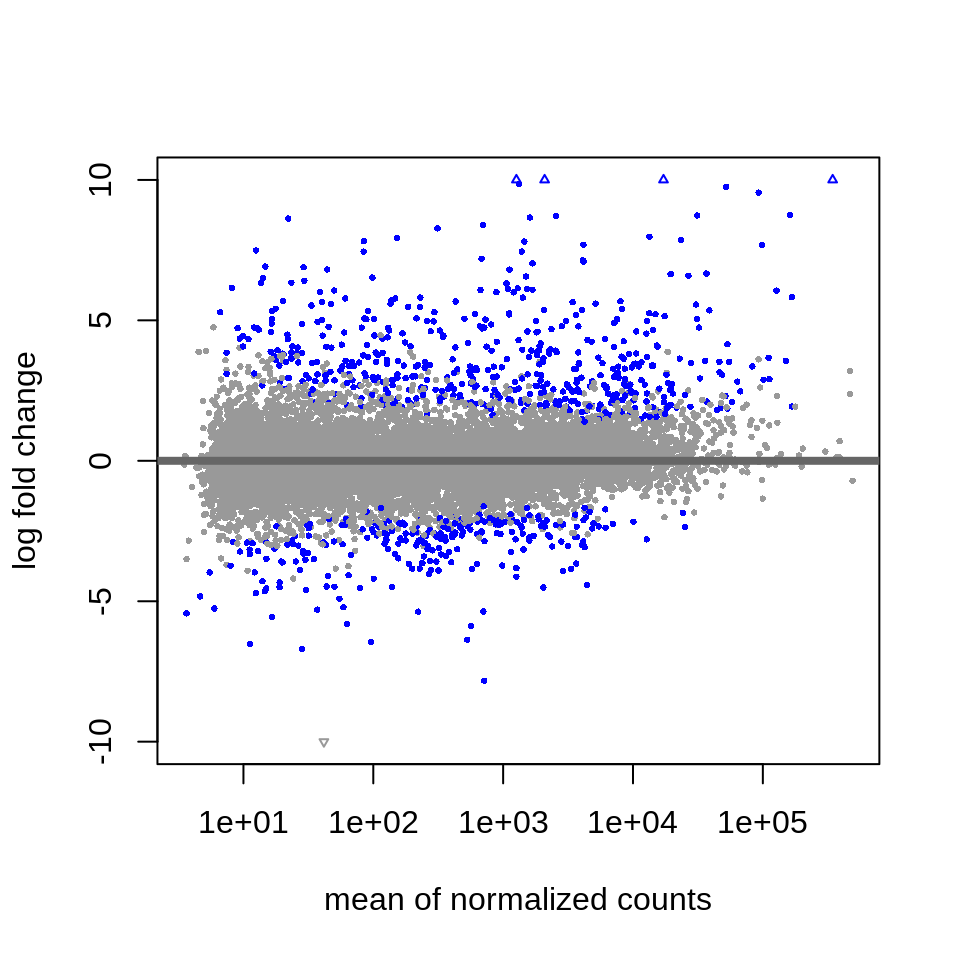
\includegraphics{/Users/lee.s/fluentGenomics/docs/fluentGenomics_files/figure-latex/ma-plot-1} 

}

\caption{Visualization of \emph{DESeq2} results as an ``MA plot''. Genes that have
an adjusted \emph{p-value} below 0.01 are colored red.}\label{fig:ma-plot}
\end{figure}

We now output the results as a \emph{GRanges} object, and due to the conventions of
\emph{plyranges}, we construct a new column called \texttt{gene\_id} from the row names of
the results. Each row now contains the genomic region (\texttt{seqnames}, \texttt{start},
\texttt{end}, \texttt{strand}) along with corresponding metadata columns (the \texttt{gene\_id} and
the results of the test). Note that \emph{tximeta} has correctly identified the
reference genome as ``hg38'', and this has also been added to the \emph{GRanges} along
the results columns. This kind of book-keeping is vital once overlap operations
are performed to ensure that \emph{plyranges} is not comparing across incompatible
genomes.

\begin{Shaded}
\begin{Highlighting}[]
\KeywordTok{suppressPackageStartupMessages}\NormalTok{(}\KeywordTok{library}\NormalTok{(plyranges))}
\NormalTok{de_genes <-}\StringTok{ }\KeywordTok{results}\NormalTok{(dds,}
                    \DataTypeTok{contrast=}\KeywordTok{c}\NormalTok{(}\StringTok{"condition"}\NormalTok{,}\StringTok{"IFNg"}\NormalTok{,}\StringTok{"naive"}\NormalTok{),}
                    \DataTypeTok{lfcThreshold=}\DecValTok{1}\NormalTok{,}
                    \DataTypeTok{format=}\StringTok{"GRanges"}\NormalTok{) }\OperatorTok
\StringTok{  }\KeywordTok{names_to_column}\NormalTok{(}\StringTok{"gene_id"}\NormalTok{)}
\NormalTok{de_genes}
\end{Highlighting}
\end{Shaded}

\begin{verbatim}
## GRanges object with 17806 ranges and 7 metadata columns:
##           seqnames              ranges strand |            gene_id
##              <Rle>           <IRanges>  <Rle> |        <character>
##       [1]     chrX 100627109-100639991      - | ENSG00000000003.14
##       [2]    chr20   50934867-50958555      - | ENSG00000000419.12
##       [3]     chr1 169849631-169894267      - | ENSG00000000457.13
##       [4]     chr1 169662007-169854080      + | ENSG00000000460.16
##       [5]     chr1   27612064-27635277      - | ENSG00000000938.12
##       ...      ...                 ...    ... .                ...
##   [17802]    chr10   84167228-84172093      - |  ENSG00000285972.1
##   [17803]     chr6   63572012-63583587      + |  ENSG00000285976.1
##   [17804]    chr16   57177349-57181390      + |  ENSG00000285979.1
##   [17805]     chr8 103398658-103501895      - |  ENSG00000285982.1
##   [17806]    chr10   12563151-12567351      + |  ENSG00000285994.1
##                   baseMean     log2FoldChange              lfcSE
##                  <numeric>          <numeric>          <numeric>
##       [1] 171.570646163445 -0.282245015065582  0.300571026277417
##       [2] 967.751278980391 0.0391222756936352 0.0859707605047955
##       [3] 682.432885098654    1.2846178585311  0.196906721741941
##       [4] 262.963397841117  -1.47187616421189  0.218691645887265
##       [5] 2660.10225731917  0.675478091290521  0.236053041372838
##       ...              ...                ...                ...
##   [17802] 10.0474624496157  0.548451844773876  0.444318686394084
##   [17803] 4586.34616821518 -0.033929582570062  0.188004977365846
##   [17804] 14.2965310090402  0.312347650582085  0.522699844356108
##   [17805] 27.7629588245413  0.994518742790125   1.58237312176743
##   [17806] 6.60408582708505   0.25399752352481    0.5957511892896
##                        stat             pvalue              padj
##                   <numeric>          <numeric>         <numeric>
##       [1]                 0                  1                 1
##       [2]                 0                  1                 1
##       [3]  1.44544511235177  0.148332899695748                 1
##       [4] -2.15772377722715 0.0309493141635637 0.409727500369082
##       [5]                 0                  1                 1
##       ...               ...                ...               ...
##   [17802]                 0                  1                 1
##   [17803]                 0                  1                 1
##   [17804]                 0                  1                 1
##   [17805]                 0                  1                 1
##   [17806]                 0                  1                 1
##   -------
##   seqinfo: 25 sequences (1 circular) from hg38 genome
\end{verbatim}

From this, we can restrict the results to those that meet our FDR threshold and
select (and rename) the metadata columns we're interested in:

\begin{Shaded}
\begin{Highlighting}[]
\NormalTok{de_genes <-}\StringTok{ }\NormalTok{de_genes }\OperatorTok
\StringTok{  }\KeywordTok{filter}\NormalTok{(padj }\OperatorTok{<}\StringTok{ }\FloatTok{0.01}\NormalTok{) }\OperatorTok
\StringTok{  }\KeywordTok{select}\NormalTok{(gene_id, }\DataTypeTok{de_log2FC =}\NormalTok{ log2FoldChange, }\DataTypeTok{de_padj =}\NormalTok{ padj)}
\end{Highlighting}
\end{Shaded}

We now wish to extract genes for which there is evidence that the LFC is \emph{not}
large. We perform this test by specifying an LFC threshold and an alternative
hypothesis (\texttt{altHypothesis}) that the LFC is less than the threshold in
absolute value. To visualize the result of this test, you can run \texttt{results}
without \texttt{format="GRanges"}, and pass this object to \texttt{plotMA} as before. We
label these genes as \texttt{other\_genes} and later as ``non-DE genes'', for comparison
with our \texttt{de\_genes} set.

\begin{Shaded}
\begin{Highlighting}[]
\NormalTok{other_genes <-}\StringTok{ }\KeywordTok{results}\NormalTok{(dds,}
                       \DataTypeTok{contrast=}\KeywordTok{c}\NormalTok{(}\StringTok{"condition"}\NormalTok{,}\StringTok{"IFNg"}\NormalTok{,}\StringTok{"naive"}\NormalTok{),}
                       \DataTypeTok{lfcThreshold=}\DecValTok{1}\NormalTok{,}
                       \DataTypeTok{altHypothesis=}\StringTok{"lessAbs"}\NormalTok{,}
                       \DataTypeTok{format=}\StringTok{"GRanges"}\NormalTok{) }\OperatorTok
\StringTok{  }\KeywordTok{filter}\NormalTok{(padj }\OperatorTok{<}\StringTok{ }\FloatTok{0.01}\NormalTok{) }\OperatorTok
\StringTok{  }\KeywordTok{names_to_column}\NormalTok{(}\StringTok{"gene_id"}\NormalTok{) }\OperatorTok
\StringTok{  }\NormalTok{dplyr}\OperatorTok{::}\KeywordTok{select}\NormalTok{(gene_id,}
                \DataTypeTok{de_log2FC =}\NormalTok{ log2FoldChange,}
                \DataTypeTok{de_padj =}\NormalTok{ padj)}
\end{Highlighting}
\end{Shaded}

\hypertarget{atac-seq-peak-differential-abundance-analysis}{%
\subsection{ATAC-seq peak differential abundance analysis}\label{atac-seq-peak-differential-abundance-analysis}}

The following section describes the process we have used for generating a
\emph{GRanges} object of differential peaks from the ATAC-seq data in K Alasoo et al. (\protect\hyperlink{ref-alasoo}{2018}).

The code chunks for the remainder of this section are not run.

For assessing differential accessibility, we run \emph{limma} (G. K. Smyth \protect\hyperlink{ref-Smyth2004}{2004}), and
generate the a summary of LFCs and adjusted p-values for the peaks:

\begin{Shaded}
\begin{Highlighting}[]
\KeywordTok{library}\NormalTok{(limma)}
\NormalTok{design <-}\StringTok{ }\KeywordTok{model.matrix}\NormalTok{(}\OperatorTok{~}\NormalTok{donor }\OperatorTok{+}\StringTok{ }\NormalTok{condition, }\KeywordTok{colData}\NormalTok{(atac))}
\NormalTok{fit <-}\StringTok{ }\KeywordTok{lmFit}\NormalTok{(}\KeywordTok{assay}\NormalTok{(atac), design)}
\NormalTok{fit <-}\StringTok{ }\KeywordTok{eBayes}\NormalTok{(fit)}
\NormalTok{idx <-}\StringTok{ }\KeywordTok{which}\NormalTok{(}\KeywordTok{colnames}\NormalTok{(fit}\OperatorTok{$}\NormalTok{coefficients) }\OperatorTok{==}\StringTok{ "conditionIFNg"}\NormalTok{)}
\NormalTok{tt <-}\StringTok{ }\KeywordTok{topTable}\NormalTok{(fit, }\DataTypeTok{coef=}\NormalTok{idx, }\DataTypeTok{sort.by=}\StringTok{"none"}\NormalTok{, }\DataTypeTok{n=}\KeywordTok{nrow}\NormalTok{(atac))}
\end{Highlighting}
\end{Shaded}

We now take the \texttt{rowRanges} of the \emph{SummarizedExperiment} and attach the LFCs
and adjusted p-values from \emph{limma}, so that we can consider the overlap with
differential expression. Note that we set the genome build to ``hg38'' and
restyle the chromosome information to use the ``UCSC'' style (e.g.~``chr1'',
``chr2'', etc.). Again, we know the genome build from the Zenodo entry for the
ATAC-seq data.

\begin{Shaded}
\begin{Highlighting}[]
\NormalTok{atac_peaks <-}\StringTok{ }\KeywordTok{rowRanges}\NormalTok{(atac) }\OperatorTok
\StringTok{  }\KeywordTok{remove_names}\NormalTok{() }\OperatorTok
\StringTok{  }\KeywordTok{mutate}\NormalTok{(}
    \DataTypeTok{da_log2FC =}\NormalTok{ tt}\OperatorTok{$}\NormalTok{logFC,}
    \DataTypeTok{da_padj =}\NormalTok{ tt}\OperatorTok{$}\NormalTok{adj.P.Val}
\NormalTok{  ) }\OperatorTok
\StringTok{  }\KeywordTok{set_genome_info}\NormalTok{(}\DataTypeTok{genome =} \StringTok{"hg38"}\NormalTok{)}

\KeywordTok{seqlevelsStyle}\NormalTok{(atac_peaks) <-}\StringTok{ "UCSC"}
\end{Highlighting}
\end{Shaded}

The final \emph{GRanges} object containing the DA peaks is included in the workflow
package and can be loaded as follows:

\begin{Shaded}
\begin{Highlighting}[]
\KeywordTok{library}\NormalTok{(fluentGenomics)}
\NormalTok{peaks}
\end{Highlighting}
\end{Shaded}

\begin{verbatim}
## GRanges object with 296220 ranges and 3 metadata columns:
##            seqnames              ranges strand |          peak_id
##               <Rle>           <IRanges>  <Rle> |      <character>
##        [1]     chr1          9979-10668      * |      ATAC_peak_1
##        [2]     chr1         10939-11473      * |      ATAC_peak_2
##        [3]     chr1         15505-15729      * |      ATAC_peak_3
##        [4]     chr1         21148-21481      * |      ATAC_peak_4
##        [5]     chr1         21864-22067      * |      ATAC_peak_5
##        ...      ...                 ...    ... .              ...
##   [296216]     chrX 155896572-155896835      * | ATAC_peak_296216
##   [296217]     chrX 155958507-155958646      * | ATAC_peak_296217
##   [296218]     chrX 156016760-156016975      * | ATAC_peak_296218
##   [296219]     chrX 156028551-156029422      * | ATAC_peak_296219
##   [296220]     chrX 156030135-156030785      * | ATAC_peak_296220
##                     da_log2FC              da_padj
##                     <numeric>            <numeric>
##        [1]  0.266185396736073 9.10672732956434e-05
##        [2]   0.32217712436691 2.03434717570469e-05
##        [3] -0.574159538548115 3.41707743345703e-08
##        [4]  -1.14706617895329 8.22298606986521e-26
##        [5] -0.896143162633654 4.79452571676397e-11
##        ...                ...                  ...
##   [296216] -0.834628897017445  1.3354605397165e-11
##   [296217] -0.147537281935847    0.313014754316915
##   [296218] -0.609732301631964 3.62338775135558e-09
##   [296219] -0.347678474957794 6.94823191242968e-06
##   [296220]  0.492442459200901 7.07663984067763e-13
##   -------
##   seqinfo: 23 sequences from hg38 genome; no seqlengths
\end{verbatim}

\hypertarget{integrate-ranges}{%
\section{Integrate ranges}\label{integrate-ranges}}

\hypertarget{finding-overlaps-with-plyranges}{%
\subsection{\texorpdfstring{Finding overlaps with \emph{plyranges}}{Finding overlaps with plyranges}}\label{finding-overlaps-with-plyranges}}

We have already used \emph{plyranges} a number of times above, to \texttt{filter},
\texttt{mutate}, and \texttt{select} on \emph{GRanges} objects, as well as ensuring the correct
genome annotation and style has been used. The \emph{plyranges} package provides a
grammar for performing transformations of genomic data (Lee, Cook, and Lawrence \protect\hyperlink{ref-Lee2019}{2019}). Computations
resulting from compositions of \emph{plyranges} ``verbs'' are performed using
underlying, highly optimized range operations in the \emph{GenomicRanges} package
(Lawrence et al. \protect\hyperlink{ref-granges}{2013}).

For the overlap analysis, we filter the annotated peaks to have a nominal FDR
bound of 1\%.

\begin{Shaded}
\begin{Highlighting}[]
\NormalTok{da_peaks <-}\StringTok{ }\NormalTok{peaks }\OperatorTok
\StringTok{  }\KeywordTok{filter}\NormalTok{(da_padj }\OperatorTok{<}\StringTok{ }\FloatTok{0.01}\NormalTok{)}
\end{Highlighting}
\end{Shaded}

We now have \emph{GRanges} objects that contain DE genes, genes without strong
signal of DE, and DA peaks. We are ready to answer the question: is there an
enrichment of DA ATAC-seq peaks in the vicinity of DE genes compared to genes
without sufficient DE signal?

\hypertarget{down-sampling-non-differentially-expressed-genes}{%
\subsection{Down sampling non-differentially expressed genes}\label{down-sampling-non-differentially-expressed-genes}}

As \emph{plyranges} is built on top of \emph{dplyr}, it implements methods for many of
its verbs for \emph{GRanges} objects. Here we can use \texttt{slice} to randomly sample the
rows of the \texttt{other\_genes}. The \texttt{sample.int} function will generate random
samples of size equal to the number of DE-genes from the number of rows in
\texttt{other\_genes}:

\begin{Shaded}
\begin{Highlighting}[]
\NormalTok{size <-}\StringTok{ }\KeywordTok{length}\NormalTok{(de_genes)}
\KeywordTok{slice}\NormalTok{(other_genes, }\KeywordTok{sample.int}\NormalTok{(}\KeywordTok{n}\NormalTok{(), size))}
\end{Highlighting}
\end{Shaded}

\begin{verbatim}
## GRanges object with 749 ranges and 3 metadata columns:
##         seqnames              ranges strand |            gene_id
##            <Rle>           <IRanges>  <Rle> |        <character>
##     [1]     chr9 128819651-128829821      - | ENSG00000198917.12
##     [2]     chr4       958887-986895      - | ENSG00000145214.13
##     [3]     chr7   32916815-32943176      - | ENSG00000205763.13
##     [4]    chr15   74598500-74645414      + | ENSG00000179335.18
##     [5]    chr19   43996896-44002836      - |  ENSG00000266921.1
##     ...      ...                 ...    ... .                ...
##   [745]     chr2 231732425-231786272      - | ENSG00000156973.13
##   [746]    chr13 112686769-112689815      - |  ENSG00000274922.1
##   [747]     chr9   93576407-93679587      + | ENSG00000197724.10
##   [748]     chr8 143597835-143603224      + |  ENSG00000179886.5
##   [749]    chr17   81666364-81673904      + | ENSG00000185298.12
##                    de_log2FC              de_padj
##                    <numeric>            <numeric>
##     [1]   0.0125804041562409 8.20768195120974e-09
##     [2]    -0.27201809520893 3.08085205452332e-07
##     [3]   0.0781232048133288  8.0547909233735e-07
##     [4]    0.120324259003472 1.36912324994382e-13
##     [5] 0.000218895401361497  0.00485688559956773
##     ...                  ...                  ...
##   [745]    0.498346851622183  0.00118441064644543
##   [746]    0.169372408097565  0.00120695857265466
##   [747]   -0.252325705825331 5.95814403873254e-11
##   [748]    0.108005256969665 5.27090615809167e-06
##   [749]   0.0592693549492427 1.73737397840478e-06
##   -------
##   seqinfo: 25 sequences (1 circular) from hg38 genome
\end{verbatim}

We can repeat this many times to create many samples via \texttt{replicate}. By
replicating the sub-sampling multiple times, we minimize the variance on the
enrichment statistics induced by the sampling process.

\begin{Shaded}
\begin{Highlighting}[]
\CommentTok{# set a seed for the results}
\KeywordTok{set.seed}\NormalTok{(}\DecValTok{2019-08-02}\NormalTok{)}
\NormalTok{boot_genes <-}\StringTok{ }\KeywordTok{replicate}\NormalTok{(}\DecValTok{10}\NormalTok{,}
                        \KeywordTok{slice}\NormalTok{(other_genes, }\KeywordTok{sample.int}\NormalTok{(}\KeywordTok{n}\NormalTok{(), size)),}
                        \DataTypeTok{simplify =} \OtherTok{FALSE}\NormalTok{)}
\end{Highlighting}
\end{Shaded}

This creates a list of \emph{GRanges} objects as a list, and we can bind these
together using the \texttt{bind\_ranges} function. This function creates a new column
called ``resample'' on the result that identifies each of the input \emph{GRanges}
objects:

\begin{Shaded}
\begin{Highlighting}[]
\NormalTok{boot_genes <-}\StringTok{ }\KeywordTok{bind_ranges}\NormalTok{(boot_genes, }\DataTypeTok{.id =} \StringTok{"resample"}\NormalTok{)}
\end{Highlighting}
\end{Shaded}

Similarly, we can then combine the \texttt{boot\_genes} \emph{GRanges}, with the DE
\emph{GRanges} object. As the resample column was not present on the DE \emph{GRanges}
object, this is given a missing value which we recode to a 0 using \texttt{mutate()}

\begin{Shaded}
\begin{Highlighting}[]
\NormalTok{all_genes <-}\StringTok{ }\KeywordTok{bind_ranges}\NormalTok{(}
  \DataTypeTok{de=}\NormalTok{de_genes,}
  \DataTypeTok{not_de =}\NormalTok{ boot_genes,}
  \DataTypeTok{.id=}\StringTok{"origin"}
\NormalTok{) }\OperatorTok
\StringTok{  }\KeywordTok{mutate}\NormalTok{(}
    \DataTypeTok{origin =} \KeywordTok{factor}\NormalTok{(origin, }\KeywordTok{c}\NormalTok{(}\StringTok{"not_de"}\NormalTok{, }\StringTok{"de"}\NormalTok{)),}
    \DataTypeTok{resample =} \KeywordTok{ifelse}\NormalTok{(}\KeywordTok{is.na}\NormalTok{(resample), 0L, }\KeywordTok{as.integer}\NormalTok{(resample))}
\NormalTok{  )}
\NormalTok{all_genes}
\end{Highlighting}
\end{Shaded}

\begin{verbatim}
## GRanges object with 8239 ranges and 5 metadata columns:
##          seqnames              ranges strand |            gene_id
##             <Rle>           <IRanges>  <Rle> |        <character>
##      [1]     chr1 196651878-196747504      + | ENSG00000000971.15
##      [2]     chr6   46129993-46146699      + |  ENSG00000001561.6
##      [3]     chr4   17577192-17607972      + | ENSG00000002549.12
##      [4]     chr7 150800403-150805120      + |  ENSG00000002933.8
##      [5]     chr4   15778275-15853230      + | ENSG00000004468.12
##      ...      ...                 ...    ... .                ...
##   [8235]    chr17   43527844-43579620      - | ENSG00000175832.12
##   [8236]    chr17   18260534-18266552      + | ENSG00000177427.12
##   [8237]    chr20   63895182-63936031      + | ENSG00000101152.10
##   [8238]     chr1   39081316-39487177      + | ENSG00000127603.25
##   [8239]     chr8   41577187-41625001      + | ENSG00000158669.11
##                   de_log2FC              de_padj  resample   origin
##                   <numeric>            <numeric> <integer> <factor>
##      [1]   4.98711071930695 1.37057050625117e-13         0       de
##      [2]   1.92721595378787  3.1747750217733e-05         0       de
##      [3]   2.93372501059128  2.0131038573066e-11         0       de
##      [4]   3.16721751137972 1.07359906028984e-08         0       de
##      [5]   5.40894352968188 4.82904694023763e-18         0       de
##      ...                ...                  ...       ...      ...
##   [8235] -0.240918426099239  0.00991611085813261        10   not_de
##   [8236] -0.166059030395757  9.1205141062356e-05        10   not_de
##   [8237]  0.250538999517482 1.74084544559733e-09        10   not_de
##   [8238] -0.385053503003028  0.00265539384929076        10   not_de
##   [8239]  0.155922038318879  2.9637514745875e-17        10   not_de
##   -------
##   seqinfo: 25 sequences (1 circular) from hg38 genome
\end{verbatim}

\hypertarget{expanding-genomic-coordinates-around-the-transcription-start-site}{%
\subsection{Expanding genomic coordinates around the transcription start site}\label{expanding-genomic-coordinates-around-the-transcription-start-site}}

Now we would like to modify our gene ranges so they contain the 10 kilobases on
either side of their transcription start site (TSS). There are many ways one
could do this, but we prefer an approach via the anchoring methods in
\emph{plyranges}. Because there is a mutual dependence between the start, end,
width, and strand of a \emph{GRanges} object, we define anchors to fix one of
\texttt{start} and \texttt{end}, while modifying the \texttt{width}. As an example, to extract just
the TSS, we can anchor by the 5' end of the range and modify the width of the
range to equal 1.

\begin{Shaded}
\begin{Highlighting}[]
\NormalTok{all_genes <-}\StringTok{ }\NormalTok{all_genes }\OperatorTok
\StringTok{  }\KeywordTok{anchor_5p}\NormalTok{() }\OperatorTok
\StringTok{  }\KeywordTok{mutate}\NormalTok{(}\DataTypeTok{width =} \DecValTok{1}\NormalTok{)}
\end{Highlighting}
\end{Shaded}

Anchoring by the 5' end of a range will fix the \texttt{end} of negatively stranded
ranges, and fix the \texttt{start} of positively stranded ranges.

We can then repeat the same pattern but this time using \texttt{anchor\_center()} to
tell \emph{plyranges} that we are making the TSS the midpoint of a range that has
total width of 20kb, or 10kb both upstream and downstream of the TSS.

\begin{Shaded}
\begin{Highlighting}[]
\NormalTok{all_genes <-}\StringTok{ }\NormalTok{all_genes }\OperatorTok
\StringTok{  }\KeywordTok{anchor_center}\NormalTok{() }\OperatorTok
\StringTok{  }\KeywordTok{mutate}\NormalTok{(}\DataTypeTok{width=}\DecValTok{2}\OperatorTok{*}\FloatTok{1e4}\NormalTok{)}
\end{Highlighting}
\end{Shaded}

\hypertarget{use-overlap-joins-to-find-relative-enrichment}{%
\subsection{Use overlap joins to find relative enrichment}\label{use-overlap-joins-to-find-relative-enrichment}}

We are now ready to compute overlaps between RNA-seq genes (our DE set and
bootstrap sets) and the ATAC-seq peaks. In \emph{plyranges}, overlaps are defined as
joins between two \emph{GRanges} objects: a \emph{left} and a \emph{right} \emph{GRanges} object.
In an overlap join, a match is any range on the \emph{left} \emph{GRanges} that is
overlapped by the \emph{right} \emph{GRanges}. One powerful aspect of the overlap joins
is that the result maintains all (metadata) columns from each of the \emph{left} and
\emph{right} ranges which makes downstream summaries easy to compute.

To combine the DE genes with the DA peaks, we perform a left overlap join. This
returns to us the \texttt{all\_genes} ranges (potentially with duplication), but with
the metadata columns from those overlapping DA peaks. For any gene that has no
overlaps, the DA peak columns will have \texttt{NA}'s.

\begin{Shaded}
\begin{Highlighting}[]
\NormalTok{genes_olap_peaks <-}\StringTok{ }\NormalTok{all_genes }\OperatorTok
\StringTok{  }\KeywordTok{join_overlap_left}\NormalTok{(da_peaks)}
\NormalTok{genes_olap_peaks}
\end{Highlighting}
\end{Shaded}

\begin{verbatim}
## GRanges object with 27766 ranges and 8 metadata columns:
##           seqnames              ranges strand |            gene_id
##              <Rle>           <IRanges>  <Rle> |        <character>
##       [1]     chr1 196641878-196661877      + | ENSG00000000971.15
##       [2]     chr6   46119993-46139992      + |  ENSG00000001561.6
##       [3]     chr4   17567192-17587191      + | ENSG00000002549.12
##       [4]     chr4   17567192-17587191      + | ENSG00000002549.12
##       [5]     chr4   17567192-17587191      + | ENSG00000002549.12
##       ...      ...                 ...    ... .                ...
##   [27762]     chr1   39071316-39091315      + | ENSG00000127603.25
##   [27763]     chr1   39071316-39091315      + | ENSG00000127603.25
##   [27764]     chr8   41567187-41587186      + | ENSG00000158669.11
##   [27765]     chr8   41567187-41587186      + | ENSG00000158669.11
##   [27766]     chr8   41567187-41587186      + | ENSG00000158669.11
##                    de_log2FC              de_padj  resample   origin
##                    <numeric>            <numeric> <integer> <factor>
##       [1]   4.98711071930695 1.37057050625117e-13         0       de
##       [2]   1.92721595378787  3.1747750217733e-05         0       de
##       [3]   2.93372501059128  2.0131038573066e-11         0       de
##       [4]   2.93372501059128  2.0131038573066e-11         0       de
##       [5]   2.93372501059128  2.0131038573066e-11         0       de
##       ...                ...                  ...       ...      ...
##   [27762] -0.385053503003028  0.00265539384929076        10   not_de
##   [27763] -0.385053503003028  0.00265539384929076        10   not_de
##   [27764]  0.155922038318879  2.9637514745875e-17        10   not_de
##   [27765]  0.155922038318879  2.9637514745875e-17        10   not_de
##   [27766]  0.155922038318879  2.9637514745875e-17        10   not_de
##                    peak_id          da_log2FC              da_padj
##                <character>          <numeric>            <numeric>
##       [1]  ATAC_peak_21236 -0.546582189082724 0.000115273676444232
##       [2] ATAC_peak_231183   1.45329684862127  9.7322474682763e-17
##       [3] ATAC_peak_193578  0.222371496904895 3.00939005719989e-11
##       [4] ATAC_peak_193579 -0.281615137872819 7.99888515457195e-05
##       [5] ATAC_peak_193580  0.673705317951604 7.60042918890061e-15
##       ...              ...                ...                  ...
##   [27762]   ATAC_peak_5357  -1.05823584693303 3.69051674661467e-16
##   [27763]   ATAC_peak_5358  -1.31411238041643 6.44280493172654e-26
##   [27764] ATAC_peak_263396 -0.904080135059089 8.19576651692093e-13
##   [27765] ATAC_peak_263397  0.364737985368599 2.08834835864614e-08
##   [27766] ATAC_peak_263399  0.317386691052334 1.20088116314111e-08
##   -------
##   seqinfo: 25 sequences (1 circular) from hg38 genome
\end{verbatim}

Now we can ask, how many DA peaks are near DE genes relative to ``other'' non-DE
genes? A gene may appear more than once in \texttt{genes\_olap\_peaks}, because
multiple peaks may overlap a single gene, or because we have re-sampled the
same gene more than once, or a combination of these two cases.

For each gene (that is the combination of chromosome, the start, end, and
strand), and the ``origin'' (DE vs not-DE) we can compute the distinct number of
peaks for each gene and the maximum peak based on LFC. This is achieved via
\texttt{reduce\_ranges\_directed}, which allows an aggregation to result in a \emph{GRanges}
object via merging neighboring genomic regions. The use of the directed suffix
indicates we're maintaining strand information. In this case, we are simply
merging ranges (genes) via the groups we mentioned above. We also have to
account for the number of resamples we have performed when counting if there
are any peaks, to ensure we do not double count the same peak:

\begin{Shaded}
\begin{Highlighting}[]
\NormalTok{gene_peak_max_lfc <-}\StringTok{ }\NormalTok{genes_olap_peaks }\OperatorTok
\StringTok{  }\KeywordTok{group_by}\NormalTok{(gene_id, origin)  }\OperatorTok
\StringTok{  }\KeywordTok{reduce_ranges_directed}\NormalTok{(}
    \DataTypeTok{peak_count =} \KeywordTok{sum}\NormalTok{(}\OperatorTok{!}\KeywordTok{is.na}\NormalTok{(da_padj)) }\OperatorTok{/}\StringTok{ }\KeywordTok{n_distinct}\NormalTok{(resample),}
    \DataTypeTok{peak_max_lfc =} \KeywordTok{max}\NormalTok{(}\KeywordTok{abs}\NormalTok{(da_log2FC))}
\NormalTok{  )}
\end{Highlighting}
\end{Shaded}

We can then filter genes if they have any peaks and compare the peak fold
changes between non-DE and DE genes using a boxplot:

\begin{Shaded}
\begin{Highlighting}[]
\KeywordTok{library}\NormalTok{(ggplot2)}
\NormalTok{gene_peak_max_lfc }\OperatorTok
\StringTok{  }\KeywordTok{filter}\NormalTok{(peak_count }\OperatorTok{>}\StringTok{ }\DecValTok{0}\NormalTok{) }\OperatorTok
\StringTok{  }\KeywordTok{as.data.frame}\NormalTok{() }\OperatorTok
\StringTok{  }\KeywordTok{ggplot}\NormalTok{(}\KeywordTok{aes}\NormalTok{(origin, peak_max_lfc)) }\OperatorTok{+}
\StringTok{  }\KeywordTok{geom_boxplot}\NormalTok{()}
\end{Highlighting}
\end{Shaded}

\begin{figure}

{\centering 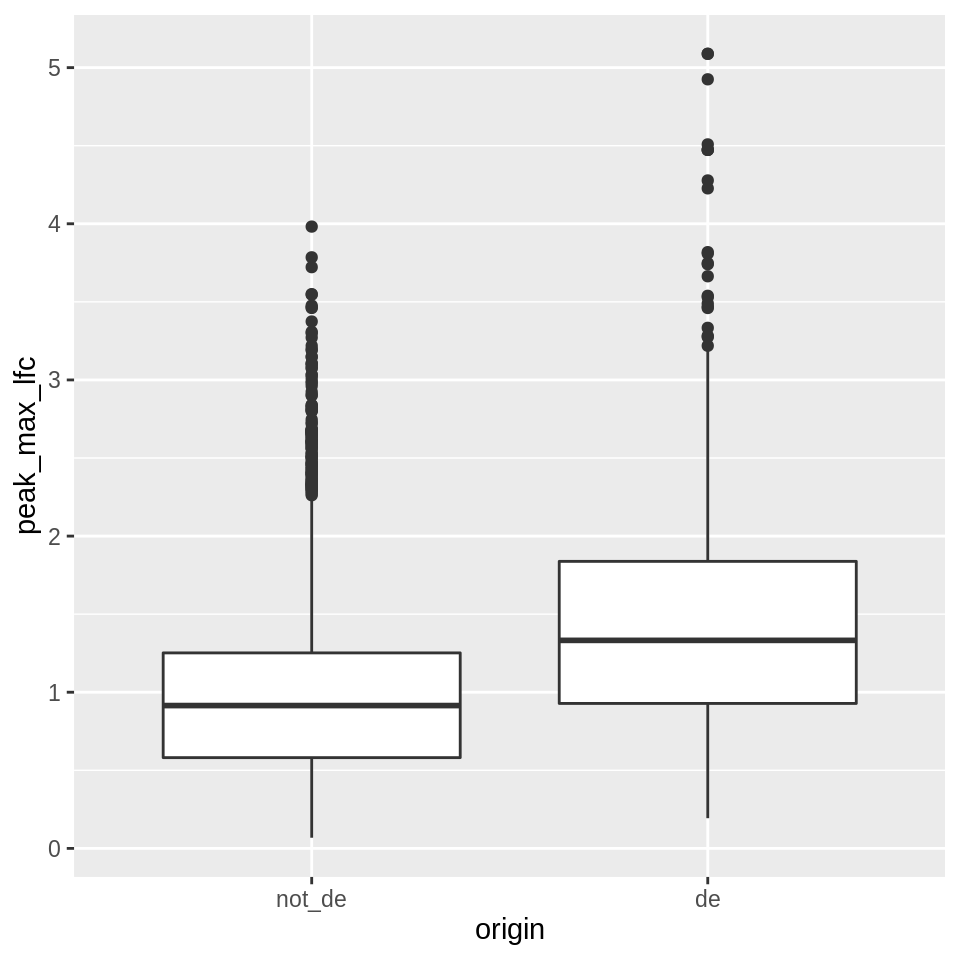
\includegraphics{/Users/lee.s/fluentGenomics/docs/fluentGenomics_files/figure-latex/boxplot-1} 

}

\caption{A boxplot of maximum LFCs for DA peaks for DE genes compared to
non-DE genes where genes have at least one DA peak.}\label{fig:boxplot}
\end{figure}

In general, the DE genes have larger maximum DA fold changes relative to the
non-DE genes.

Next we examine how thresholds on the DA LFC modify the enrichment we observe
of DA peaks near DE or non-DE genes. First, we want to know how the number of
peaks within DE genes and non-DE genes change as we change threshold values on
the peak LFC. As an example, we could compute this by arbitrarily chosen LFC
thresholds of 1 or 2 as follows:

\begin{Shaded}
\begin{Highlighting}[]
\NormalTok{origin_peak_lfc <-}\StringTok{ }\NormalTok{genes_olap_peaks }\OperatorTok
\StringTok{  }\KeywordTok{group_by}\NormalTok{(origin) }\OperatorTok
\StringTok{  }\KeywordTok{summarize}\NormalTok{(}
    \DataTypeTok{peak_count =} \KeywordTok{sum}\NormalTok{(}\OperatorTok{!}\KeywordTok{is.na}\NormalTok{(da_padj)) }\OperatorTok{/}\StringTok{ }\KeywordTok{n_distinct}\NormalTok{(resample),}
    \DataTypeTok{lfc1_peak_count =}\KeywordTok{sum}\NormalTok{(}\KeywordTok{abs}\NormalTok{(da_log2FC) }\OperatorTok{>}\StringTok{ }\DecValTok{1}\NormalTok{, }\DataTypeTok{na.rm=}\OtherTok{TRUE}\NormalTok{)}\OperatorTok{/}\StringTok{ }\KeywordTok{n_distinct}\NormalTok{(resample),}
    \DataTypeTok{lfc2_peak_count =} \KeywordTok{sum}\NormalTok{(}\KeywordTok{abs}\NormalTok{(da_log2FC) }\OperatorTok{>}\StringTok{ }\DecValTok{2}\NormalTok{, }\DataTypeTok{na.rm=}\OtherTok{TRUE}\NormalTok{)}\OperatorTok{/}\StringTok{ }\KeywordTok{n_distinct}\NormalTok{(resample)}
\NormalTok{  )}
\NormalTok{origin_peak_lfc}
\end{Highlighting}
\end{Shaded}

\begin{verbatim}
## DataFrame with 2 rows and 4 columns
##     origin peak_count lfc1_peak_count lfc2_peak_count
##   <factor>  <numeric>       <numeric>       <numeric>
## 1   not_de     2391.8           369.5            32.5
## 2       de       3416            1097             234
\end{verbatim}

Here we see that DE genes tend to have more DA peaks near them, and that the
number of DA peaks decreases as we increase the DA LFC threshold (as expected).
We now show how to compute the ratio of peak counts from DE compared to non-DE
genes, so we can see how this ratio changes for various DA LFC thresholds.

For all variables except for the \texttt{origin} column we divide the first row's
values by the second row, which will be the enrichment of peaks in DE genes
compared to other genes. This requires us to reshape the summary table from
long form back to wide form using the \emph{tidyr} package. First we pivot the
results of the \texttt{peak\_count} columns into name-value pairs, then pivot again to
place values into the \texttt{origin} column. Then we create a new column with the
relative enrichment:

\begin{Shaded}
\begin{Highlighting}[]
\NormalTok{origin_peak_lfc }\OperatorTok
\StringTok{  }\KeywordTok{as.data.frame}\NormalTok{() }\OperatorTok
\StringTok{  }\NormalTok{tidyr}\OperatorTok{::}\KeywordTok{pivot_longer}\NormalTok{(}\DataTypeTok{cols =} \OperatorTok{-}\NormalTok{origin) }\OperatorTok
\StringTok{  }\NormalTok{tidyr}\OperatorTok{::}\KeywordTok{pivot_wider}\NormalTok{(}\DataTypeTok{names_from =}\NormalTok{ origin, }\DataTypeTok{values_from =}\NormalTok{ value) }\OperatorTok
\StringTok{  }\KeywordTok{mutate}\NormalTok{(}\DataTypeTok{enrichment =}\NormalTok{ de }\OperatorTok{/}\StringTok{ }\NormalTok{not_de)}
\end{Highlighting}
\end{Shaded}

\begin{verbatim}
## # A tibble: 3 x 4
##   name            not_de    de enrichment
##   <chr>            <dbl> <dbl>      <dbl>
## 1 peak_count      2392.   3416       1.43
## 2 lfc1_peak_count  370.   1097       2.97
## 3 lfc2_peak_count   32.5   234       7.2
\end{verbatim}

The above table shows that relative enrichment increases for a larger LFC
threshold.

Due to the one-to-many mappings of genes to peaks, it is unknown if we have the
same number of DE genes participating or less, as we increase the threshold on
the DA LFC. We can examine the number of genes with overlapping DA peaks at
various thresholds by grouping and aggregating twice. First, the number of
peaks that meet the thresholds are computed within each gene, origin, and
resample group. Second, within the origin column, we compute the total number
of peaks that meet the DA LFC threshold and the number of genes that have more
than zero peaks (again averaging over the number of resamples).

\begin{Shaded}
\begin{Highlighting}[]
\NormalTok{genes_olap_peaks }\OperatorTok
\StringTok{  }\KeywordTok{group_by}\NormalTok{(gene_id, origin, resample) }\OperatorTok
\StringTok{  }\KeywordTok{reduce_ranges_directed}\NormalTok{(}
    \DataTypeTok{lfc1 =} \KeywordTok{sum}\NormalTok{(}\KeywordTok{abs}\NormalTok{(da_log2FC) }\OperatorTok{>}\StringTok{ }\DecValTok{1}\NormalTok{, }\DataTypeTok{na.rm=}\OtherTok{TRUE}\NormalTok{),}
    \DataTypeTok{lfc2 =} \KeywordTok{sum}\NormalTok{(}\KeywordTok{abs}\NormalTok{(da_log2FC) }\OperatorTok{>}\StringTok{ }\DecValTok{2}\NormalTok{, }\DataTypeTok{na.rm=}\OtherTok{TRUE}\NormalTok{)}
\NormalTok{  ) }\OperatorTok
\StringTok{  }\KeywordTok{group_by}\NormalTok{(origin) }\OperatorTok
\StringTok{  }\KeywordTok{summarize}\NormalTok{(}
    \DataTypeTok{lfc1_gene_count =} \KeywordTok{sum}\NormalTok{(lfc1 }\OperatorTok{>}\StringTok{ }\DecValTok{0}\NormalTok{) }\OperatorTok{/}\StringTok{ }\KeywordTok{n_distinct}\NormalTok{(resample),}
    \DataTypeTok{lfc1_peak_count =} \KeywordTok{sum}\NormalTok{(lfc1) }\OperatorTok{/}\StringTok{ }\KeywordTok{n_distinct}\NormalTok{(resample),}
    \DataTypeTok{lfc2_gene_count =} \KeywordTok{sum}\NormalTok{(lfc2 }\OperatorTok{>}\StringTok{ }\DecValTok{0}\NormalTok{) }\OperatorTok{/}\StringTok{ }\KeywordTok{n_distinct}\NormalTok{(resample),}
    \DataTypeTok{lfc2_peak_count =} \KeywordTok{sum}\NormalTok{(lfc2) }\OperatorTok{/}\StringTok{ }\KeywordTok{n_distinct}\NormalTok{(resample)}
\NormalTok{  )}
\end{Highlighting}
\end{Shaded}

\begin{verbatim}
## DataFrame with 2 rows and 5 columns
##     origin lfc1_gene_count lfc1_peak_count lfc2_gene_count lfc2_peak_count
##   <factor>       <numeric>       <numeric>       <numeric>       <numeric>
## 1   not_de           271.2           369.5            30.3            32.5
## 2       de             515            1097             151             234
\end{verbatim}

To do this for many thresholds is cumbersome and would create a lot of
duplicate code. Instead we create a single function called
\texttt{count\_above\_threshold} that accepts a variable and a vector of thresholds, and
computes the sum of the absolute value of the variable for each element in the
\texttt{thresholds} vector.

\begin{Shaded}
\begin{Highlighting}[]
\NormalTok{count_if_above_threshold <-}\StringTok{ }\ControlFlowTok{function}\NormalTok{(var, thresholds) \{}
  \KeywordTok{lapply}\NormalTok{(thresholds, }\ControlFlowTok{function}\NormalTok{(.) }\KeywordTok{sum}\NormalTok{(}\KeywordTok{abs}\NormalTok{(var) }\OperatorTok{>}\StringTok{ }\NormalTok{., }\DataTypeTok{na.rm =} \OtherTok{TRUE}\NormalTok{))}
\NormalTok{\}}
\end{Highlighting}
\end{Shaded}

The above function will compute the counts for any arbitrary threshold, so we
can apply it over possible LFC thresholds of interest. We choose a grid of one
hundred thresholds based on the range of absolute LFC values in the \texttt{da\_peaks}
\emph{GRanges} object:

\begin{Shaded}
\begin{Highlighting}[]
\NormalTok{thresholds <-}\StringTok{ }\NormalTok{da_peaks }\OperatorTok
\StringTok{  }\KeywordTok{mutate}\NormalTok{(}\DataTypeTok{abs_lfc =} \KeywordTok{abs}\NormalTok{(da_log2FC)) }\OperatorTok
\StringTok{  }\KeywordTok{with}\NormalTok{(}
    \KeywordTok{seq}\NormalTok{(}\KeywordTok{min}\NormalTok{(abs_lfc), }\KeywordTok{max}\NormalTok{(abs_lfc), }\DataTypeTok{length.out =} \DecValTok{100}\NormalTok{)}
\NormalTok{  )}
\end{Highlighting}
\end{Shaded}

The peak counts for each threshold are computed as a new list-column called
\texttt{value}. First, the \emph{GRanges} object has been grouped by the gene, origin, and
the number of resamples columns. Then we aggregate over those columns, so each
row will contain the peak counts for all of the thresholds for a gene, origin,
and resample. We also maintain another list-column that contains the threshold
values.

\begin{Shaded}
\begin{Highlighting}[]
\NormalTok{genes_peak_all_thresholds <-}\StringTok{ }\NormalTok{genes_olap_peaks }\OperatorTok
\StringTok{  }\KeywordTok{group_by}\NormalTok{(gene_id, origin, resample) }\OperatorTok
\StringTok{  }\KeywordTok{reduce_ranges_directed}\NormalTok{(}
    \DataTypeTok{value =} \KeywordTok{count_if_above_threshold}\NormalTok{(da_log2FC, thresholds),}
    \DataTypeTok{threshold =} \KeywordTok{list}\NormalTok{(thresholds)}
\NormalTok{  )}
\NormalTok{genes_peak_all_thresholds}
\end{Highlighting}
\end{Shaded}

\begin{verbatim}
## GRanges object with 8239 ranges and 5 metadata columns:
##          seqnames              ranges strand |            gene_id   origin
##             <Rle>           <IRanges>  <Rle> |        <character> <factor>
##      [1]     chr1 196641878-196661877      + | ENSG00000000971.15       de
##      [2]     chr6   46119993-46139992      + |  ENSG00000001561.6       de
##      [3]     chr4   17567192-17587191      + | ENSG00000002549.12       de
##      [4]     chr7 150790403-150810402      + |  ENSG00000002933.8       de
##      [5]     chr4   15768275-15788274      + | ENSG00000004468.12       de
##      ...      ...                 ...    ... .                ...      ...
##   [8235]    chr17   43569620-43589619      - | ENSG00000175832.12   not_de
##   [8236]    chr17   18250534-18270533      + | ENSG00000177427.12   not_de
##   [8237]    chr20   63885182-63905181      + | ENSG00000101152.10   not_de
##   [8238]     chr1   39071316-39091315      + | ENSG00000127603.25   not_de
##   [8239]     chr8   41567187-41587186      + | ENSG00000158669.11   not_de
##           resample         value
##          <integer> <IntegerList>
##      [1]         0     1,1,1,...
##      [2]         0     1,1,1,...
##      [3]         0     6,6,6,...
##      [4]         0     4,4,4,...
##      [5]         0  11,11,11,...
##      ...       ...           ...
##   [8235]        10     1,1,1,...
##   [8236]        10     3,3,2,...
##   [8237]        10     5,5,5,...
##   [8238]        10     3,3,3,...
##   [8239]        10     3,3,3,...
##                                                           threshold
##                                                       <NumericList>
##      [1] 0.0658243106359027,0.118483961449043,0.171143612262182,...
##      [2] 0.0658243106359027,0.118483961449043,0.171143612262182,...
##      [3] 0.0658243106359027,0.118483961449043,0.171143612262182,...
##      [4] 0.0658243106359027,0.118483961449043,0.171143612262182,...
##      [5] 0.0658243106359027,0.118483961449043,0.171143612262182,...
##      ...                                                        ...
##   [8235] 0.0658243106359027,0.118483961449043,0.171143612262182,...
##   [8236] 0.0658243106359027,0.118483961449043,0.171143612262182,...
##   [8237] 0.0658243106359027,0.118483961449043,0.171143612262182,...
##   [8238] 0.0658243106359027,0.118483961449043,0.171143612262182,...
##   [8239] 0.0658243106359027,0.118483961449043,0.171143612262182,...
##   -------
##   seqinfo: 25 sequences (1 circular) from hg38 genome
\end{verbatim}

Now we can expand these list-columns into a long \emph{GRanges} object using the
\texttt{expand\_ranges()} function. This function will unlist the \texttt{value} and
\texttt{threshold} columns and lengthen the resulting \emph{GRanges} object. To compute
the peak and gene counts for each threshold, we apply the same summarization as
before:

\begin{Shaded}
\begin{Highlighting}[]
\NormalTok{origin_peak_all_thresholds <-}\StringTok{ }\NormalTok{genes_peak_all_thresholds }\OperatorTok
\StringTok{  }\KeywordTok{expand_ranges}\NormalTok{() }\OperatorTok
\StringTok{  }\KeywordTok{group_by}\NormalTok{(origin, threshold) }\OperatorTok
\StringTok{  }\KeywordTok{summarize}\NormalTok{(}
    \DataTypeTok{gene_count =} \KeywordTok{sum}\NormalTok{(value }\OperatorTok{>}\StringTok{ }\DecValTok{0}\NormalTok{) }\OperatorTok{/}\StringTok{ }\KeywordTok{n_distinct}\NormalTok{(resample),}
    \DataTypeTok{peak_count =} \KeywordTok{sum}\NormalTok{(value) }\OperatorTok{/}\StringTok{ }\KeywordTok{n_distinct}\NormalTok{(resample)}
\NormalTok{  )}
\NormalTok{origin_peak_all_thresholds}
\end{Highlighting}
\end{Shaded}

\begin{verbatim}
## DataFrame with 200 rows and 4 columns
##       origin          threshold gene_count peak_count
##     <factor>          <numeric>  <numeric>  <numeric>
## 1     not_de 0.0658243106359027        708     2391.4
## 2     not_de  0.118483961449043      698.8     2320.6
## 3     not_de  0.171143612262182      686.2     2178.6
## 4     not_de  0.223803263075322      672.4     1989.4
## 5     not_de  0.276462913888462      650.4     1785.8
## ...      ...                ...        ...        ...
## 196       de   5.06849113788419          2          2
## 197       de   5.12115078869733          0          0
## 198       de   5.17381043951047          0          0
## 199       de   5.22647009032361          0          0
## 200       de   5.27912974113675          0          0
\end{verbatim}

Again we can compute the relative enrichment in LFCs in the same manner as
before, by pivoting the results to long form then back to wide form to compute
the enrichment. We visualize the peak enrichment changes of DE genes relative
to other genes as a line chart:

\begin{Shaded}
\begin{Highlighting}[]
\NormalTok{origin_threshold_counts <-}\StringTok{ }\NormalTok{origin_peak_all_thresholds }\OperatorTok
\StringTok{  }\KeywordTok{as.data.frame}\NormalTok{() }\OperatorTok
\StringTok{  }\NormalTok{tidyr}\OperatorTok{::}\KeywordTok{pivot_longer}\NormalTok{(}\DataTypeTok{cols =} \OperatorTok{-}\KeywordTok{c}\NormalTok{(origin, threshold),}
                      \DataTypeTok{names_to =} \KeywordTok{c}\NormalTok{(}\StringTok{"type"}\NormalTok{, }\StringTok{"var"}\NormalTok{),}
                      \DataTypeTok{names_sep =} \StringTok{"_"}\NormalTok{,}
                      \DataTypeTok{values_to =} \StringTok{"count"}\NormalTok{) }\OperatorTok
\StringTok{  }\KeywordTok{select}\NormalTok{(}\OperatorTok{-}\NormalTok{var)}

\NormalTok{origin_threshold_counts }\OperatorTok
\StringTok{  }\KeywordTok{filter}\NormalTok{(type }\OperatorTok{==}\StringTok{ "peak"}\NormalTok{) }\OperatorTok
\StringTok{  }\NormalTok{tidyr}\OperatorTok{::}\KeywordTok{pivot_wider}\NormalTok{(}\DataTypeTok{names_from =}\NormalTok{ origin, }\DataTypeTok{values_from =}\NormalTok{ count) }\OperatorTok
\StringTok{  }\KeywordTok{mutate}\NormalTok{(}\DataTypeTok{enrichment =}\NormalTok{  de }\OperatorTok{/}\StringTok{ }\NormalTok{not_de) }\OperatorTok
\StringTok{  }\KeywordTok{ggplot}\NormalTok{(}\KeywordTok{aes}\NormalTok{(}\DataTypeTok{x =}\NormalTok{ threshold, }\DataTypeTok{y =}\NormalTok{ enrichment)) }\OperatorTok{+}
\StringTok{  }\KeywordTok{geom_line}\NormalTok{() }\OperatorTok{+}
\StringTok{  }\KeywordTok{labs}\NormalTok{(}\DataTypeTok{x =} \StringTok{"logFC threshold"}\NormalTok{, }\DataTypeTok{y =} \StringTok{"Relative Enrichment"}\NormalTok{)}
\end{Highlighting}
\end{Shaded}

\begin{verbatim}
## Warning: Removed 4 row(s) containing missing values (geom_path).
\end{verbatim}

\begin{figure}

{\centering 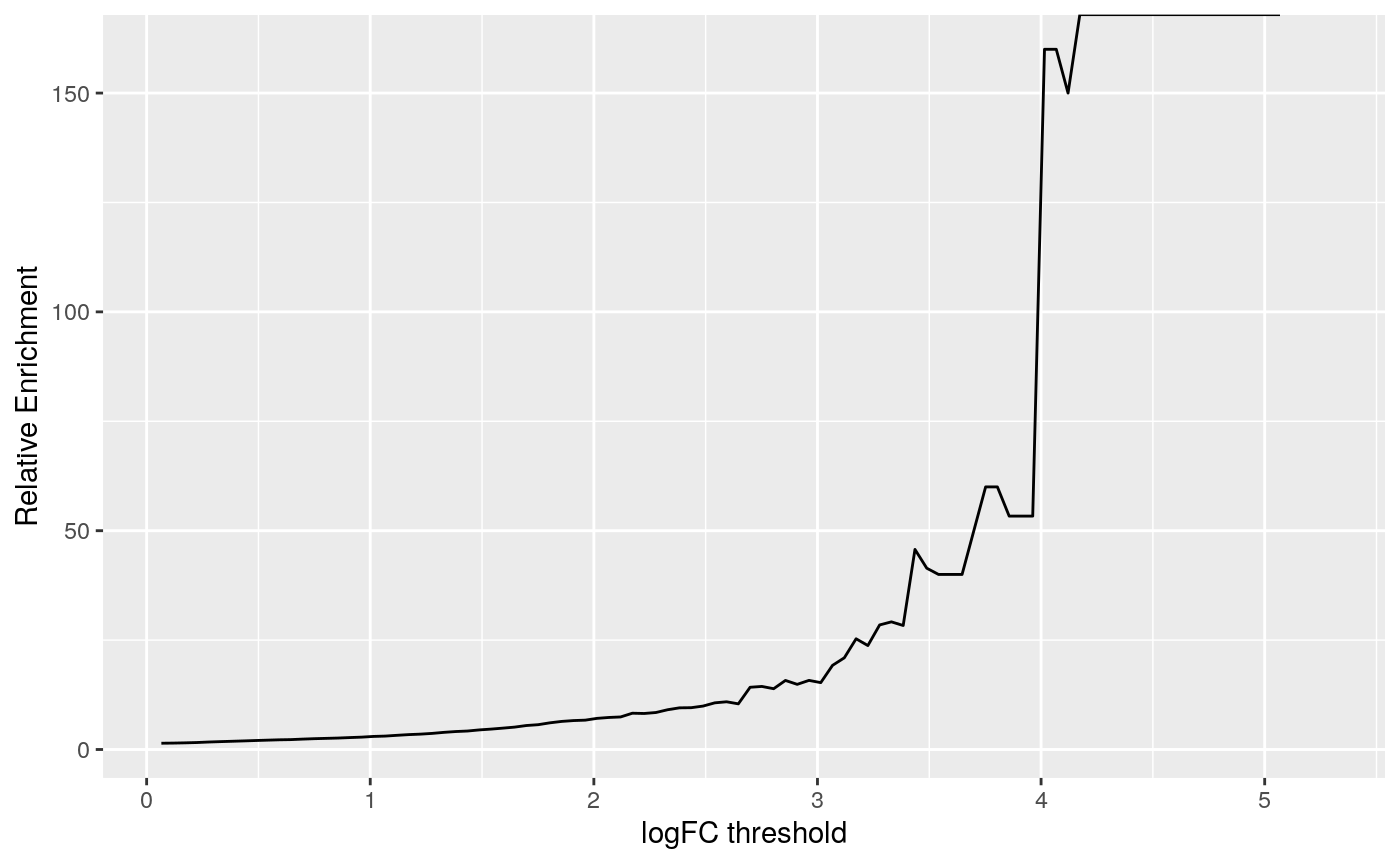
\includegraphics{/Users/lee.s/fluentGenomics/docs/fluentGenomics_files/figure-latex/line-chart-1} 

}

\caption{A line chart displaying how relative enrichment of DA peaks
change between DE genes compared to non-DE genes as the absolute DA LFC
threshold increases.}\label{fig:line-chart}
\end{figure}

We computed the sum of DA peaks near the DE genes, for increasing LFC
thresholds on the accessibility change. As we increased the threshold, the
number of total peaks went down (likewise the mean number of DA peaks per
gene). It is also likely the number of DE genes with a DA peak nearby with such
a large change went down. We can investigate this with a plot that summarizes
many of the aspects underlying the enrichment plot above.

\begin{Shaded}
\begin{Highlighting}[]
\NormalTok{origin_threshold_counts }\OperatorTok
\StringTok{  }\KeywordTok{ggplot}\NormalTok{(}\KeywordTok{aes}\NormalTok{(}\DataTypeTok{x =}\NormalTok{ threshold,}
             \DataTypeTok{y =}\NormalTok{ count }\OperatorTok{+}\StringTok{ }\DecValTok{1}\NormalTok{,}
             \DataTypeTok{color =}\NormalTok{ origin,}
             \DataTypeTok{linetype =}\NormalTok{ type)) }\OperatorTok{+}
\StringTok{  }\KeywordTok{geom_line}\NormalTok{() }\OperatorTok{+}
\StringTok{  }\KeywordTok{scale_y_log10}\NormalTok{()}
\end{Highlighting}
\end{Shaded}

\begin{figure}

{\centering 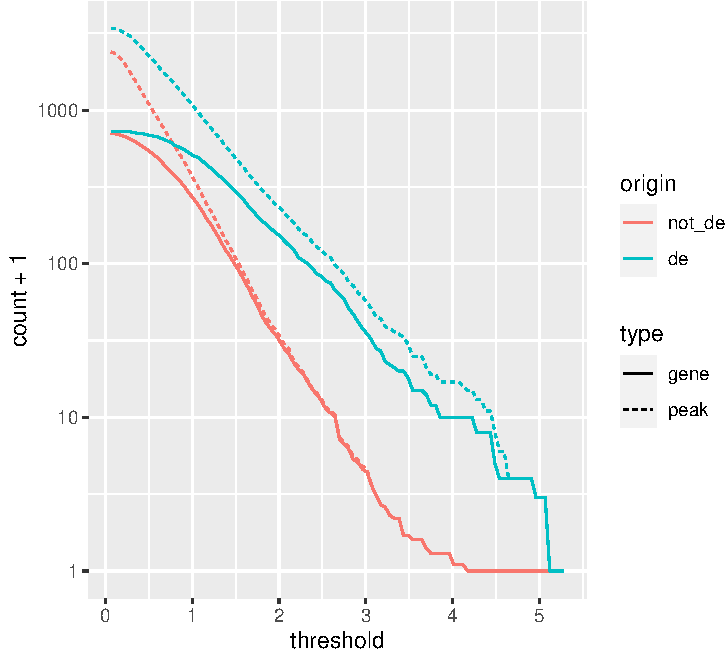
\includegraphics{/Users/lee.s/fluentGenomics/docs/fluentGenomics_files/figure-latex/line-chart2-1} 

}

\caption{A line chart displaying how gene and peak counts change as the
absolute DA LFC threshold increases. Lines are colored according to whether
they represent a gene that is DE or not. Note the x-axis is on a \(\log_{10}\)
scale.}\label{fig:line-chart2}
\end{figure}

\hypertarget{discussion}{%
\section{Discussion}\label{discussion}}

We have shown that by using \emph{plyranges} and \emph{tximeta} (with support of
Bioconductor and \emph{tidyverse} ecosystems) we can fluently iterate through the
biological data science workflow: from import, through to modeling, and data
integration.

There are several further steps that would be interesting to perform in this
analysis; for example, we could modify window size around the TSS to see how it
affects enrichment, and vary the FDR cut-offs for both the DE gene and DA peak
sets. We could also have computed variance in addition to the mean of the
bootstrap set, and so drawn an interval around the enrichment line.

Finally, our workflow illustrates the benefits of using appropriate data
abstractions provided by Bioconductor such as the \emph{SummarizedExperiment} and
\emph{GRanges}. These abstractions provide users with a mental model of their
experimental data and are the building blocks for constructing the modular and
iterative analyses we have shown here. Consequently, we have been able to
interoperate many decoupled R packages (from both Bioconductor and the
tidyverse) to construct a seamless end-to-end workflow that is far too
specialized for a single monolithic tool.

\hypertarget{software-availability}{%
\section{Software Availability}\label{software-availability}}

The workflow materials, including this article can be fully reproduced
following the instructions found at the Github repository
\href{https://github.com/sa-lee/fluentGenomics}{sa-lee/fluentGenomics}. Moreover,
the development version of the workflow and all downstream dependencies can be
installed using the \texttt{BiocManager} package by running:

\begin{Shaded}
\begin{Highlighting}[]
\CommentTok{# development version from Github}
\NormalTok{BiocManager}\OperatorTok{::}\KeywordTok{install}\NormalTok{(}\StringTok{"sa-lee/fluentGenomics"}\NormalTok{)}
\CommentTok{# version available from Bioconductor}
\NormalTok{BiocManager}\OperatorTok{::}\KeywordTok{install}\NormalTok{(}\StringTok{"fluentGenomics"}\NormalTok{)}
\end{Highlighting}
\end{Shaded}

This article and the analyses were performed with R (R Core Team \protect\hyperlink{ref-baser}{2019}) using the
\emph{rmarkdown} (Allaire et al. \protect\hyperlink{ref-rmarkdown}{2019}), and \emph{knitr} (Xie \protect\hyperlink{ref-knitr}{2019}, \protect\hyperlink{ref-xie2015}{2015}) packages.

\hypertarget{session-info}{%
\subsection{Session Info}\label{session-info}}

\begin{Shaded}
\begin{Highlighting}[]
\KeywordTok{sessionInfo}\NormalTok{()}
\end{Highlighting}
\end{Shaded}

\begin{verbatim}
## R version 3.6.1 (2019-07-05)
## Platform: x86_64-apple-darwin15.6.0 (64-bit)
## Running under: macOS Mojave 10.14.6
## 
## Matrix products: default
## BLAS:   /System/Library/Frameworks/Accelerate.framework/Versions/A/Frameworks/vecLib.framework/Versions/A/libBLAS.dylib
## LAPACK: /Library/Frameworks/R.framework/Versions/3.6/Resources/lib/libRlapack.dylib
## 
## locale:
## [1] en_AU.UTF-8/en_AU.UTF-8/en_AU.UTF-8/C/en_AU.UTF-8/en_AU.UTF-8
## 
## attached base packages:
## [1] parallel  stats4    stats     graphics  grDevices utils     datasets 
## [8] methods   base     
## 
## other attached packages:
##  [1] ggplot2_3.3.0.9000          plyranges_1.7.8            
##  [3] DESeq2_1.26.0               GenomicFeatures_1.38.0     
##  [5] AnnotationDbi_1.48.0        SummarizedExperiment_1.16.0
##  [7] DelayedArray_0.12.1         BiocParallel_1.20.0        
##  [9] matrixStats_0.55.0          Biobase_2.46.0             
## [11] GenomicRanges_1.38.0        GenomeInfoDb_1.22.0        
## [13] IRanges_2.20.1              S4Vectors_0.24.1           
## [15] BiocGenerics_0.32.0         readr_1.3.1                
## [17] dplyr_0.8.3                 tximeta_1.4.2              
## [19] fluentGenomics_0.0.5        rmarkdown_2.0              
## 
## loaded via a namespace (and not attached):
##   [1] colorspace_1.4-1         rprojroot_1.3-2          htmlTable_1.13.3        
##   [4] XVector_0.26.0           base64enc_0.1-3          rstudioapi_0.10         
##   [7] farver_2.0.3             bit64_0.9-7              fansi_0.4.1             
##  [10] xml2_1.2.2               splines_3.6.1            tximport_1.14.0         
##  [13] geneplotter_1.64.0       knitr_1.27               zeallot_0.1.0           
##  [16] Formula_1.2-3            jsonlite_1.6             Rsamtools_2.2.1         
##  [19] annotate_1.64.0          cluster_2.1.0            dbplyr_1.4.2            
##  [22] png_0.1-7                compiler_3.6.1           httr_1.4.1              
##  [25] backports_1.1.5          assertthat_0.2.1         Matrix_1.2-18           
##  [28] lazyeval_0.2.2           cli_2.0.1                acepack_1.4.1           
##  [31] htmltools_0.4.0          prettyunits_1.1.0        tools_3.6.1             
##  [34] gtable_0.3.0             glue_1.3.1               GenomeInfoDbData_1.2.2  
##  [37] rappdirs_0.3.1           Rcpp_1.0.3               vctrs_0.2.1             
##  [40] Biostrings_2.54.0        rtracklayer_1.46.0       xfun_0.12               
##  [43] stringr_1.4.0            lifecycle_0.1.0          ensembldb_2.10.2        
##  [46] XML_3.99-0.3             zlibbioc_1.32.0          scales_1.1.0            
##  [49] hms_0.5.3                ProtGenerics_1.18.0      AnnotationFilter_1.10.0 
##  [52] RColorBrewer_1.1-2       yaml_2.2.0               curl_4.3                
##  [55] memoise_1.1.0            gridExtra_2.3            biomaRt_2.42.0          
##  [58] rpart_4.1-15             hunspell_3.0             latticeExtra_0.6-29     
##  [61] stringi_1.4.5            RSQLite_2.2.0            genefilter_1.68.0       
##  [64] checkmate_1.9.4          rlang_0.4.2              pkgconfig_2.0.3         
##  [67] commonmark_1.7           bitops_1.0-6             evaluate_0.14           
##  [70] lattice_0.20-38          purrr_0.3.3              labeling_0.3            
##  [73] GenomicAlignments_1.22.1 htmlwidgets_1.5.1        bit_1.1-15.1            
##  [76] tidyselect_0.2.5         here_0.1                 magrittr_1.5            
##  [79] bookdown_0.16            R6_2.4.1                 spelling_2.1            
##  [82] Hmisc_4.3-0              DBI_1.1.0                withr_2.1.2             
##  [85] pillar_1.4.3             foreign_0.8-73           survival_3.1-8          
##  [88] RCurl_1.98-1.1           nnet_7.3-12              tibble_2.1.3            
##  [91] crayon_1.3.4             utf8_1.1.4               BiocFileCache_1.10.2    
##  [94] jpeg_0.1-8.1             progress_1.2.2           locfit_1.5-9.1          
##  [97] grid_3.6.1               data.table_1.12.8        blob_1.2.1              
## [100] digest_0.6.23            xtable_1.8-4             tidyr_1.0.0             
## [103] openssl_1.4.1            munsell_0.5.0            askpass_1.1
\end{verbatim}

\hypertarget{author-contributions}{%
\subsection{Author Contributions}\label{author-contributions}}

All authors contributed to the writing and development of the workflow.

\hypertarget{competing-interests}{%
\subsection{Competing interests}\label{competing-interests}}

The authors declare that they have no competing interests.

\hypertarget{funding}{%
\subsection{Funding}\label{funding}}

SL is supported by an Australian Government Research Training Program (RTP)
scholarship with a top up scholarship from CSL Limited.

MIL's contribution is supported by NIH grant R01 HG009937.

\textbf{I confirm that the funders had no role in study design, data collection and
analysis, decision to publish, or preparation of the manuscript.}

\hypertarget{acknowledgements}{%
\subsection{Acknowledgements}\label{acknowledgements}}

The authors would like to thank all participants of the Bioconductor 2019 and
BiocAsia 2019 conferences who attended and provided feedback on early versions
of this workflow paper.

\hypertarget{references}{%
\section*{References}\label{references}}
\addcontentsline{toc}{section}{References}

\hypertarget{refs}{}
\leavevmode\hypertarget{ref-alasoo}{}%
Alasoo, K, J Rodrigues, S Mukhopadhyay, AJ Knights, AL Mann, K Kundu, HIPSCI-Consortium, C Hale, Dougan G, and DJ Gaffney. 2018. ``Shared genetic effects on chromatin and gene expression indicate a role for enhancer priming in immune response.'' \emph{Nature Genetics} 50:424--31. \url{https://doi.org/10.1038/s41588-018-0046-7}.

\leavevmode\hypertarget{ref-alasooZenodo}{}%
Alasoo, Kaur, and Daniel Gaffney. 2017. ``Processed read counts from macrophage RNA-seq and ATAC-seq experiments.'' Zenodo. \url{https://doi.org/10.5281/zenodo.1188300}.

\leavevmode\hypertarget{ref-rmarkdown}{}%
Allaire, JJ, Yihui Xie, Jonathan McPherson, Javier Luraschi, Kevin Ushey, Aron Atkins, Hadley Wickham, Joe Cheng, Winston Chang, and Richard Iannone. 2019. \emph{Rmarkdown: Dynamic Documents for R}. \url{https://github.com/rstudio/rmarkdown}.

\leavevmode\hypertarget{ref-gencode}{}%
Frankish, A, GENCODE-consoritum, and P Flicek. 2018. ``GENCODE reference annotation for the human and mouse genomes.'' \emph{Nucleic Acids Research}. \url{https://doi.org/10.1093/nar/gky955}.

\leavevmode\hypertarget{ref-Hansen2012}{}%
Hansen, Kasper D., Rafael A. Irizarry, and Zhijin Wu. 2012. ``Removing technical variability in RNA-seq data using condition quantile normalization.'' \emph{Biostatistics} 13 (2):204--16. \url{https://doi.org/10.1093/biostatistics/kxr054}.

\leavevmode\hypertarget{ref-bioc}{}%
Huber, Wolfgang, Vincent J Carey, Robert Gentleman, Simon Anders, Marc Carlson, Benilton S Carvalho, Hector Corrada Bravo, et al. 2015. ``Orchestrating High-Throughput Genomic Analysis with Bioconductor.'' \emph{Nature Methods} 12 (2). Springer Nature:115--21. \url{https://doi.org/10.1038/nmeth.3252}.

\leavevmode\hypertarget{ref-snakemake}{}%
Köster, Johannes, and Sven Rahmann. 2012. ``Snakemake---a scalable bioinformatics workflow engine.'' \emph{Bioinformatics} 28 (19):2520--2. \url{https://doi.org/10.1093/bioinformatics/bts480}.

\leavevmode\hypertarget{ref-Law2018-f1000}{}%
Law, Charity W, Monther Alhamdoosh, Shian Su, Xueyi Dong, Luyi Tian, Gordon K Smyth, and Matthew E Ritchie. 2018. ``RNA-seq Analysis Is Easy as 1-2-3 with Limma, Glimma and edgeR.'' \emph{F1000 Research} 5 (1408). F1000 Research Limited:1408. \url{https://doi.org/10.12688/f1000research.9005.3}.

\leavevmode\hypertarget{ref-granges}{}%
Lawrence, Michael, Wolfgang Huber, Hervé Pagès, Patrick Aboyoun, Marc Carlson, Robert Gentleman, Martin Morgan, and Vincent Carey. 2013. ``Software for Computing and Annotating Genomic Ranges.'' \emph{PLoS Comput. Biol.} 9. \url{https://doi.org/10.1371/journal.pcbi.1003118}.

\leavevmode\hypertarget{ref-Lee2019}{}%
Lee, Stuart, Dianne Cook, and Michael Lawrence. 2019. ``Plyranges: A Grammar of Genomic Data Transformation.'' \emph{Genome Biology} 20 (1):4. \url{https://doi.org/10.1186/s13059-018-1597-8}.

\leavevmode\hypertarget{ref-Love2016-f1000}{}%
Love, Michael I, Simon Anders, Vladislav Kim, and Wolfgang Huber. 2016. ``RNA-Seq Workflow: Gene-Level Exploratory Analysis and Differential Expression.'' \emph{F1000 Research} 4 (1070). F1000 Research Limited:1070. \url{https://doi.org/10.12688/f1000research.7035.2}.

\leavevmode\hypertarget{ref-Love2019-tximeta}{}%
Love, Michael I, Charlotte Soneson, Peter F Hickey, Lisa K Johnson, N Tessa Pierce, Lori Shepherd, Martin Morgan, and Rob Patro. 2019. ``Tximeta: Reference Sequence Checksums for Provenance Identification in RNA-seq.'' \emph{bioRxiv}, September, 777888. \url{https://doi.org/10.1101/777888}.

\leavevmode\hypertarget{ref-Love2014}{}%
Love, Michael I., Wolfgang Huber, and Simon Anders. 2014. ``Moderated estimation of fold change and dispersion for RNA-seq data with DESeq2.'' \emph{Genome Biology} 15 (12):550. \url{https://doi.org/10.1186/s13059-014-0550-8}.

\leavevmode\hypertarget{ref-salmon}{}%
Patro, R, G Duggal, MI Love, RA Irizarry, and C Kingsford. 2017. ``Salmon Provides Fast and Bias-Aware Quantification of Transcript Expression.'' \emph{Nature Methods} 14:417--19. \url{https://doi.org/10.1038/nmeth.4197}.

\leavevmode\hypertarget{ref-baser}{}%
R Core Team. 2019. \emph{R: A Language and Environment for Statistical Computing}. Vienna, Austria: R Foundation for Statistical Computing. \url{https://www.R-project.org/}.

\leavevmode\hypertarget{ref-bcfilecache}{}%
Shepherd, Lori, and Martin Morgan. 2019. \emph{BiocFileCache: Manage Files Across Sessions}.

\leavevmode\hypertarget{ref-Smyth2004}{}%
Smyth, Gordon K. 2004. ``Linear Models and Empirical Bayes Methods for Assessing Differential Expression in Microarray Experiments.'' \emph{Statistical Applications in Genetics and Molecular Biology} 3 (1).

\leavevmode\hypertarget{ref-Soneson2015}{}%
Soneson, Charlotte, Michael I. Love, and Mark Robinson. 2015. ``Differential analyses for RNA-seq: transcript-level estimates improve gene-level inferences.'' \emph{F1000Research} 4 (1521). \url{https://doi.org/10.12688/f1000research.7563.1}.

\leavevmode\hypertarget{ref-tidyverse}{}%
Wickham, Hadley, Mara Averick, Jennifer Bryan, Winston Chang, Lucy D'Agostino McGowan, Romain François, Garrett Grolemund, et al. 2019. ``Welcome to the tidyverse.'' \emph{Journal of Open Source Software} 4 (43):1686. \url{https://doi.org/10.21105/joss.01686}.

\leavevmode\hypertarget{ref-xie2015}{}%
Xie, Yihui. 2015. \emph{Dynamic Documents with R and Knitr}. 2nd ed. Boca Raton, Florida: Chapman; Hall/CRC. \url{https://yihui.name/knitr/}.

\leavevmode\hypertarget{ref-knitr}{}%
---------. 2019. \emph{Knitr: A General-Purpose Package for Dynamic Report Generation in R}. \url{https://yihui.name/knitr/}.

\end{document}
